% \documentclass[twocolumn,3p]{elsarticle}
\documentclass[onecolumn,3p,letterpaper]{elsarticle}
% \usepackage{setspace} % added by JC 
% \doublespacing % added by JC


\usepackage{lineno} % uncomment \linenumbers after \begin{document}
\modulolinenumbers[1]

\usepackage{hyperref}

%%% MY PACKAGES %%%%%%%%%%%%%%%%%%%%%%%%%%%%%%%%%%%%%%%%%%%%%%%
\usepackage{graphicx}
% \usepackage[outdir=./]{epstopdf}
\usepackage{epstopdf}
\epstopdfsetup{update} % only regenerate pdf files when eps file is newer
\usepackage{amsmath,epsfig}

% Select what to do with todonotes: 
\usepackage[disable]{todonotes} % notes not showed
% \usepackage[draft]{todonotes}   % notes showed
\setlength{\marginparwidth}{2cm}
% \usepackage[textwidth=3.7cm]{todonotes}

\usepackage{tikz} % for flow charts
  \usetikzlibrary{shapes,arrows,positioning,shadows,calc}

\begin{filecontents*}{linereg.data}
#x y
0 4
10 24
\end{filecontents*} 

\begin{filecontents*}{linereg2.data}
#x y
2 8
8 20
\end{filecontents*}

\usepackage{draftwatermark}
\SetWatermarkLightness{0.8}
\SetWatermarkScale{4}
%%% END MY PACKAGES %%%%%%%%%%%%%%%%%%%%%%%%%%%%%%%%%%%%%%%%%%%

\journal{Remote Sensing of Environment}

\begin{document}

\linenumbers

\begin{frontmatter}

\title{Retrieval of color producing agents in Case 2 waters using Landsat 8}

% %% Group authors per affiliation:
% \author{Javier A. Concha\fnref{myfootnote}}
% \address{Radarweg 29, Amsterdam}
% \fntext[myfootnote]{Since 1880.}

%% or include affiliations in footnotes:
\author[mymainaddress]{Javier A. Concha\corref{mycorrespondingauthor}}
\cortext[mycorrespondingauthor]{Corresponding author at: Digital Imaging and Remote Sensing Laboratory,
Chester F. Carlson Center for Imaging Science,
Rochester Institute of Technology,
54 Lomb Memorial Dr., Rochester, NY 14623, USA. Tel.: +1 585 290 3145.}
\ead{jxc4005@rit.edu}

\author[mymainaddress]{John R. Schott}
\address[mymainaddress]{Rochester Institute of Technology (RIT), NY 14623, USA}
% ===============================================================
\begin{abstract}

New approaches need to be considered to solve the current high demand for color producing agent (CPA) retrievals over inland and coastal waters (Case 2 waters). 
%
Standard retrieval algorithms are known to fail over highly turbid Case 2 waters because they were developed specifically for the open ocean (Case 1 waters). 
%
Landsat 8 provides an improved signal-to-noise ratio (SNR) and a new spectral coastal aerosol band in the blue. 
%
This additional information provides means to tackle this retrieval endeavor. 
%Methods
A look-up-table (LUT) and spectrum-matching methodology was implemented to simultaneously retrieve CPAs, taking advantage of Landsat 8's new features. 
%
A LUT of spectral remote-sensing reflectances ($R_{rs}$) with different concentration of CPAs was produced using the in-water radiative transfer model Hydrolight. 
%
A model-based empirical line method (MoB-ELM) algorithm was developed to atmospherically correct the Landsat 8 imagery and allow direct comparison with the LUT of $R_{rs}$. 
%
This MoB-ELM atmospheric correction algorithm uses pseudo-invariant features (PIFs) from the image, ground-truth data and the Hydrolight model.
%Results
The retrieval algorithm was applied over two Landsat 8 scenes and shows a root mean squared error (RMSE) as a percentage of range of about $10\%$ for Chlorophyll-{\it a} and total suspended solid (TSS), and about $5\%$ for colored dissolved organic matter (CDOM) when compared with ground-truth data. The CPA concentration maps exhibit expected trends of low concentrations in clear water and higher concentrations in turbid water.
%Conclusions

These results demonstrate that the developed algorithm allows the simultaneous mapping of concentration of all CPAs in Case 2 waters and over areas where the standard algorithms are not available due to spatial resolution.
%
Therefore, this study shows that the Landsat 8 satellite can be utilized over Case 2 waters as long as a careful atmospheric correction is applied. 

\end{abstract}

\begin{keyword}
Landsat 8\sep color producing agents\sep CPAs \sep Case 2 Waters \sep retrieval
\MSC[2015] 00-01\sep  99-00
\end{keyword}

\end{frontmatter}
%%%%%%%%%%%%%%%%%%% SECTION %%%%%%%%%%%%%%%%%%%%%%%%%%%%%%%%
\section{Introduction}
The launching of a new generation of high spatial resolution satellites (e.g. Landsat 8, Sentinel 2) is opening a complete new era in the remote sensing of coastal and inland waters. New sensor specifications could meet the requirements needed to have available the same kinds of tools (e.g. Chl-{\it a} product) that the first generation of ocean color satellites, such as the Moderate Resolution Imaging Spectroradiometer (MODIS) (\cite{Esaias1998}) and the Sea-viewing Wide Field-of-view Sensor (SeaWiFS) (\cite{McClain2004}), made available for open ocean science more than a decade and half ago. The hope is to have these tools for coastal and inland waters available at a global scale and on a regular basis, similar to MODIS capabilities for open oceans. Although Landsat 8 does not have a daily frequency as MODIS does, its 16-day frequency makes it a good candidate to accomplish this endeavor, and most importantly, prepares the way for future missions with similar spatial resolution specifications (e.g. Sentinel 2, Hyperspectral Infrared Imager (HyspIRI)).

% Atmospheric correction over Case 2 water
The retrieval of color producing agents (CPA) (chlorophyll-{\it a}, sediments (or total suspended solid (TSS)) and colored dissolved organic matter (CDOM)) is in general performed in the reflectance domain, so the very first step is to perform a high quality atmospheric correction (a.k.a. atmospheric compensation) to convert the image from the satellite from radiance units to reflectance units. To perform an accurate atmospheric correction over water is extremely complex since most of the signal reaching the sensor is due to atmospheric scattering and surface reflected signal, with only a small fraction due to the signal of interest, the water-leaving signal. Therefore, it is important to perform a rigorous atmospheric correction. 

Most of the atmospheric correction algorithms for open oceans (Case 2 waters) are based on the methods developed for ocean color satellites by \cite{Gordon:1997}. These methods are based on the fact that the signal leaving the water does not contribute to the overall signal beyond the near infrared (NIR) part of the spectrum; so the signal reaching the sensor is caused only by atmospheric scattering (\cite{Gordon:1994}). This is known as the {\it black pixel assumption}. This concept can be expanded to the short wave infrared (SWIR) bands when the black pixel assumption is not valid in the NIR bands, which is the case for Case 2 and highly productive Case 1 waters (\cite{Wang:2007}). Unfortunately, most of these methods are not suitable for highly turbid coastal water, although different modifications to these algorithms have been suggested (\cite{Patt2003}).

% Landsat 8
The Landsat project has been monitoring the earth for more than four decades, being the longest uninterrupted data set available. The Landsat satellites' main mission is to image the land areas of the earth, therefore, there are typically few images available for open oceans (Case 1 water). This is one of the reasons why Landsat satellites have been underestimated by the ocean color community for the study of water bodies. In addition, the Landsat instruments have generally had broad bands and a low signal-to-noise ratio (SNR) when compared to ocean color satellites such as SeaWiFS and MODIS. However, Landsat 8 could fulfill a niche in the ocean color community for coastal and inland water body studies where a $1000m$ spatial resolution is not suitable. This is where Landsat 8 has a valuable potential for water quality studies in more optically complex water bodies (Case 2 or high productive Case 1 waters). 

Landsat 8 is the newest generation of Landsat satellites with two state-of-the-art instruments onboard, the Operational Land Imager (OLI) and the Thermal InfraRed Scanner (TIRS) (\cite{Irons:2012}). With its 12-bit quantization and improved SNR, OLI is a big improvement to the Landsat mission. In addition, OLI includes a new coastal aerosol band (Band 1: $443nm$) that increased the spectral resolution of the instrument. These improvements are the main drivers for the hypothesis that the Landsat 8 satellite could have a better performance in water quality studies than its predecessors. \cite{Roy:2014} stated this potential use of Landsat 8 for fresh and coastal water studies, mainly due to a reported SNR that exceeded expectations and the new coastal band.\todo{develop more} 

\cite*{Gerace:2013} demonstrated that the spectral coverage and radiometric resolution of OLI should dramatically improve our ability to simultaneously retrieve the CPA's concentration from water bodies. \cite{Vanhellemont2014} and \cite{Vanhellemont:2015} created a tool to apply the standard algorithm for atmospheric correction over water developed by \cite{Gordon:1994} to Landsat 8 over turbid and extremely turbid waters. In \cite{Vanhellemont:2015}, after atmospheric correction, they used the end product for detection of high concentrations of black sediments, but neither concentration values nor comparison with field measurements were reported. \cite{Franz:2015} describes an implementation of the atmospheric corrections developed by \cite{Gordon:1994} applied to Landsat 8 in the SeaWiFS Data Analysis System (SeaDAS) software package (URL: \url{http://seadas.gsfc.nasa.gov/}). A comparison of the Landsat 8's retrieved $R_{rs}$ and chlorophyll-{\it a} concentration over Chesapeake Bay with results from MODIS, SeaWiFS and {\it in situ} historical chlorophyll-{\it a} measurements is presented showing a relatively good agreement. Though again, no direct comparison to simultaneously measured values were available.
% Standard retrieval algorithms
% The standard algorithms used for chlorophyll retrieval use the methods described by \cite{OReilly2000}. Also, neural network (NN) approach \cite{Kallio:2015} that simultaneously retrieves all CPAs.


We developed a process to retrieve CPAs from Landsat 8 imagery over Case 2 waters that includes inland and coastal water. The retrieval algorithm compares water remote-sensing reflectance ($R_{rs}$) spectra with unknown concentrations to $R_{rs}$ spectra in a look-up-table (LUT) built using known concentrations. The area of study chosen for this work was the Rochester Embayment, Rochester, NY (latitude: $43^\circ18'$N and longitude: $76^\circ42'$W). An example of a Landsat 8 image showing this area of study is illustrated in \autoref{fig:L8Image130919}. This Landsat 8 image was taken on September 19, 2013 (scene LC80160302013262LGN00). This area includes Lake Ontario, the Genesee River, Irondequoit Bay and some nearby ponds (Long Pond and Cranberry Pond). This area of study was chosen because of the very wide range of constituents between the ponds and the open water in the lake, which provides a very stressing case for the retrieval.


\begin{figure}[htbp!]
  	\begin{minipage}[c]{0.48\linewidth}
    	\centering
    	\includegraphics[trim=30 350 30 350,clip,width=8cm]{./Images/WholeImage130919}
    	\centerline{(a)}\medskip
  	\end{minipage}
  	\hfill
  	\begin{minipage}[d]{0.48\linewidth}
    	\centering
    	\includegraphics[trim=0 150 30 50,width=8cm]{./Images/WaterAndDTROC}
    	\centerline{(b)}\medskip
    \end{minipage}	

    \caption{Landsat 8 image (scene LC80160302013262LGN00) acquired 09-19-2013 (a), with zoom over study region (b) showing the downtown of Rochester, NY and the Rochester Embayment. \label{fig:L8Image130919} }
\end{figure}

%%%%%%%%%%%%%%%%%%%%% SECTION %%%%%%%%%%%%%%%%%%%%%%%%%%%%%%%%
\section{Methods}
% ============================================================
\subsection{Retrieval Process Overview}
The retrieval process described in this work was first introduced by \cite*{Concha2013IGARSS} and is based on previous work done by \cite{Raqueno:2000}, \cite{Gerace:2012}, \cite{Pahlevan:2012b} and \cite{Gerace:2013}. A flow diagram of the process is illustrated in \autoref{fig:retrieval}. In short, the retrieval process works as follows. First, the radiance image from the satellite is atmospherically corrected and transformed to $R_{rs}$ spectra, as shown in the diagram. At this point the $R_{rs}$ spectra of water pixels in the scene with unknown CPAs concentrations are compared with a LUT of $R_{rs}$ spectra with known CPAs concentrations. This comparison is made by using a spectrum-matching technique (\cite{Raqueno:2000,Mobley:2005}) that calculates the root mean squared error (RMSE) to find the closest match in the LUT. The end products are maps of CPAs concentrations (see \autoref{fig:retrieval}). Each step in this retrieval process is described in more detail below.

\begin{figure}[htbp!]
	\centering
    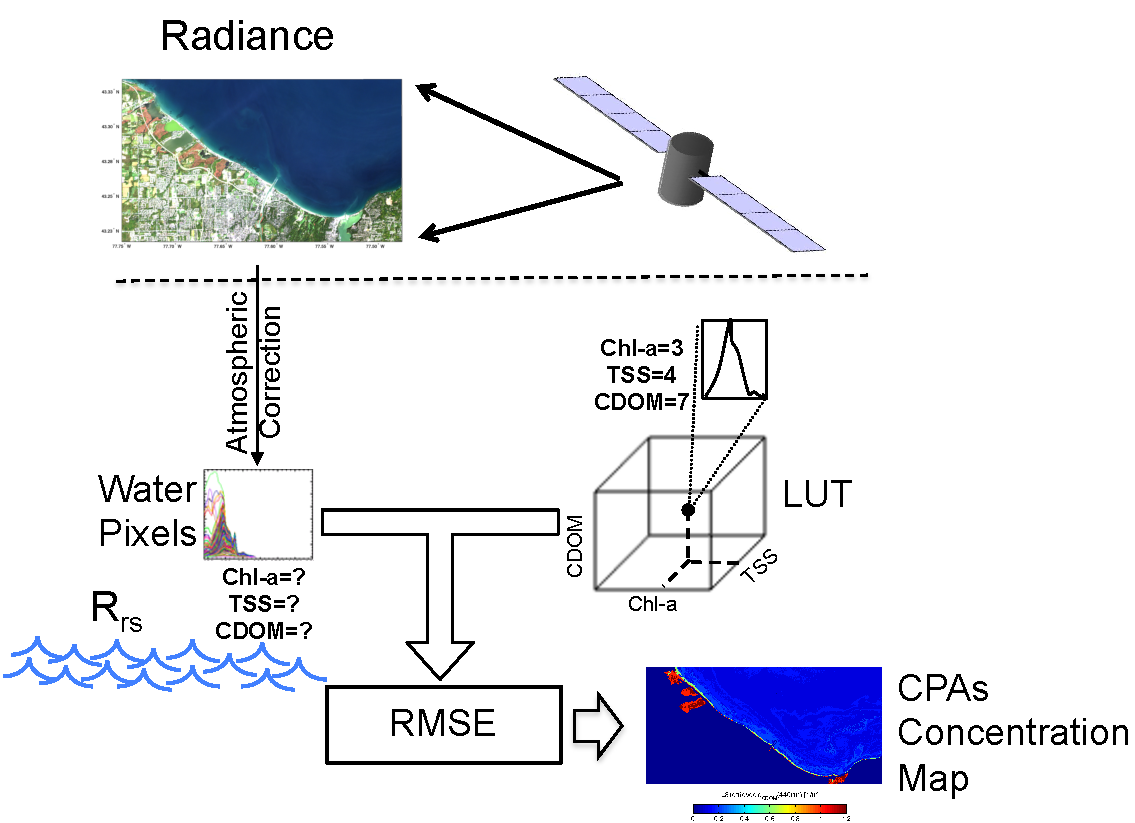
\includegraphics[height=8cm]{./Images/Retrieval_RMSE.pdf}
    \caption{Retrieval process flow diagram. The radiance image from the satellite is first corrected for atmospheric effects, having as result $R_{rs}$ spectra for each water pixel in the image. Then, a spectrum-matching methodology is used to find the closest match in the least-squared sense for the water pixels with unknown CPAs concentration in the LUT of water pixels with known CPAs concentration. The final result is a concentration map for each CPA.  \label{fig:retrieval} }
\end{figure}

% ---------------------------------------------------------------
\subsection{The MoB-ELM Atmospheric Correction}
An overview of the atmospheric correction method used in the work is described by \cite{Concha2014SPIE}, and it is explained in more detail in this paper. This is a model-based empirical line method (MoB-ELM) based on the work done for simulated OLI data by \cite{Gerace:2012}. The MoB-ELM atmospheric correction is a modified version of the traditional empirical line method (ELM) (a.k.a. empirical line fit or ELF). The ELM atmospheric correction method uses at least two pixels from the scene with known reflectance values (\cite{Schott}). It assumes that there is a linear relationship between the radiance values from the image and the reflectance values from ground-truth data. Therefore, the ELM method consists of solving the following linear regression:

\begin{equation}\label{eq:ELM} 
	L = m\cdot R_{rs} + b
\end{equation}

\noindent where $L$ is the radiance reaching the sensor, $m$ is the slope of the regression, $R_{rs}$ is the remote-sensing reflectance of the target, and $b=L_u$ is the intercept, with $L_u$ being the upwelled radiance (a.k.a. path radiance). $L$ and $R_{rs}$ in \autoref{eq:ELM} are the known radiance values from the image and the ground-truth data from the field, respectively. In order to solve for the unknown $m$ and $b$ values in \autoref{eq:ELM}, at least two pixels are needed. These two pixels are known as the {\it bright} and {\it dark} pixels because they are chosen from a bright and dark object in the scene in order to represent the whole range of values in the scene. The concept behind the traditional ELM is illustrated in \autoref{fig:ELMregression} showing a plot of $R_{rs}$ versus radiance $L$ values for the $ith$ band, $Band_{i}$. This regression is solved for each band independently. After $m$ and $b$ have been determined, the $R_{rs}$ of each water pixel in each band can be calculated from its $L$ value in the image using $R_{rs}=(L-b)/m$. Note that the ELM assumes that the atmosphere is uniform across the region of the image over which it is applied.

\begin{figure}[htb]
	\centering
% \resizebox{9cm}{!}{%
\begin{tikzpicture}[x=4ex,y=1ex]
 	%axis
	\draw (0,0) -- coordinate (x axis mid) (10,0);
    \draw (0,0) -- coordinate (y axis mid) (0,30);
 
    %labels      
	\node[below=0ex] at (8,0) {\small $Band_i~~remote-sensing~reflectance~(R_{rs})$};
	\node[rotate=90] at (-.5,23) {\small $Band_i~~Radiance~(L)$};

	\node[below=.2ex] at (-2.1,4.5) {\scriptsize $b=$offset};
	\node[below=1.4ex] at (-2.1,4.0) {\scriptsize (path radiance)};
	\draw[rotate=90,|<->|] (0,1) -- coordinate (x axis mid) (1,1);

	\node[below=0ex] at (2,15) {\small Dark Object};
	\draw[arrows=-triangle 45] (2,12.5) -- (2,9);

	\node[below=0ex] at (4,20) {\small $m=$ Slope};
	\draw[arrows=-triangle 45] (4,17.5) -- (5,14.5);

	\node[below=0ex] at (7,27) {\small Bright Object};
	\draw[arrows=-triangle 45] (7,24.5) -- (7.9,20.5);

	\node[below=0ex] at (8,9) {\small $R_{rs}=(L-b)/m$};

	%plots
	\draw plot 
		file {linereg.data};
	\draw plot[mark=*] 
		file {linereg2.data};

\end{tikzpicture}
\caption{Traditional ELM. Two pixels from the image, the bright and dark pixel, are used to solve a liner regression with a slope $m$ and offset $b$ in the $R_{rs}$, $L$ space. Once this relationship is established, each $L$ value in the image can be converted to $R_{rs}$ through $R_{rs}=(L-b)/m$. \label{fig:ELMregression}}
\end{figure}

The bright and dark objects in the scene need to be approximately uniform over at least 3-by-3 pixels (\cite{Schott}). This means that for the spatial resolution of Landsat 8, these objects have to be at least $90\times 90$ meters. This requirement is not always feasible. Additionally, it is not always possible to have ground-truth reflectance data in every satellite overpass. The MoB-ELM avoids the need for ground-truth  reflectance collection at each overpass by using pseudo-invariant features (PIFs) in the scene as the bright object and a $R_{rs}$ value from the physics-based numerical model for water, Hydrolight, for the dark object. The following sections describe the way the $L$ and $R_{rs}$ values for these two pixels are determined.

% ---------------------------------------------------------------
\subsubsection{Bright Pixel Determination}

The MoB-ELM method uses pseudo-invariant features (PIF) extraction to determine the bright pixel from the Landsat 8 image. PIFs are features in the scene that do not change their reflectivity properties drastically over time. Urban features could be considered as PIFs, and therefore, this extraction is applied over an urban area within the image. The downtown of Rochester, NY was selected as the urban area in our case (\autoref{fig:L8Image130919}). We created a PIF mask following the PIF extraction method described by \cite{Schott:1988} in order to isolate the PIFs in the Landsat 8 image. A flow diagram describing this PIF extraction method is illustrated in \autoref{fig:PIFflowchart}. This extraction method takes advantage of two facts. The first is that water is highly absorbent in the SWIR, which makes water a dark target beyond the NIR wavelengths, i.e. water has low values when compared with urban features and vegetation in the NIR. The second fact is that vegetation has a high value in the NIR when compared with the red (red edge). Therefore, a ratio between the NIR band and the red band has a high value for vegetation and a low value for urban features and water. 

The steps for the PIF extraction are the following:
\begin{enumerate}\itemsep10pt
	\item A mask that passes the urban features and vegetation, and rejects water is created (represented as Urban ON, Veget. ON and Water OFF in the left arm of \autoref{fig:PIFflowchart}). To accomplish this, the second short wave infrared band (SWIR 2) of Landsat 8 is used. A threshold is selected so that the water pixels are masked off.
	\item A mask that passes the urban features and water, and rejects vegetation is created (represented as Urban ON, Veget. OFF and Water ON in the right arm of \autoref{fig:PIFflowchart}). To accomplish this, the ratio between the NIR band and red band of Landsat 8 is thresholded so that the high values for vegetation are rejected.
	\item The previous two masks are combined using a logic $.AND.$ gate, as shown in \autoref{fig:PIFflowchart}, creating a ``PIF mask'' that rejects the vegetation and water, and only passes the urban features.
	\item The PIF mask is applied to the image, obtaining the PIF image as the result.

\end{enumerate}

\begin{figure}[htb]
  \centering
  \resizebox{10cm}{!}{%
  \begin{tikzpicture}[node distance=0.75cm, auto]
          \tikzset{
                  basenode/.style={rectangle,rounded corners,draw=black,very thick, inner sep=1em, minimum size=3em, text centered,text width=2cm},
                  productnode/.style={ellipse,rounded corners,draw=black, very thick, text centered,text width=1.5cm},
                  myarrow/.style={->,>=stealth',thick, double = black},
                  mylabel/.style={text width=7em, text centered}
          }
          % SWIR branch
          \node[basenode] (SWIR) {SWIR 2\\ Band};
          \node[basenode, below=of SWIR] (TS1) {Mask by Threshold (upward)};
          \node[align=left, right=0.0 of TS1] (C1) {Urban\\Veget.\\Water};
          \node[align=left, right=-0.15 of C1] (C2) {ON\\ON\\OFF};

          % Ratio branch
          \node[basenode, right=2.5cm of SWIR] (Ratio) {Ratio\\ NIR Band/ Red Band};
          \node[basenode, below=of Ratio] (TS2) {Mask by Threshold (downward)};
          \node[align=left, right=0.0 of TS2] (C3) {Urban\\Veget.\\Water};
          \node[align=left, right=-0.15 of C3] (C4) {ON\\OFF\\ON};

          % AND
          \path (TS1.south)--(TS2.south) node[pos=.5,below=2cm] (AND) {$.AND.$};


          % PIF Mask
          \node[basenode, below=of AND] (PIFMask){PIF Mask};
          \node[align=left, left=0.85 of PIFMask] (C5) {Urban\\Veget.\\Water};
          \node[align=left, right=-0.15 of C5] (C6) {ON\\OFF\\OFF};

          \node[basenode, below=of TS2,right=2.0cm of AND] (Image) {Image};
          \path (Image.south)--(PIFMask.east) node[below=of Image,right=2cm of PIFMask] (AND2) {$.AND.$};
          \node[basenode, right=2cm of AND2] (PIFIm){PIF Image};

          \draw[myarrow] (SWIR)--(TS1);
          \draw[myarrow] (Ratio)--(TS2);
          \draw[myarrow] (TS1)--(AND);
          \draw[myarrow] (TS2)--(AND);
          \draw[myarrow] (AND)--(PIFMask);
          \draw[myarrow] (Image)--(AND2);
          \draw[myarrow] (PIFMask)--(AND2);
          \draw[myarrow] (AND2)--(PIFIm);
  \end{tikzpicture}
  }% end resizebox
\caption{Flow chart for the PIF extraction method. Two mask are created. The first one rejects water pixel. The second mask rejects vegetation. The end mask, named PIF mask, is a combination of both previous masks that only passes the urban features. \label{fig:PIFflowchart}}
\end{figure}

Note that the urban features could change from one acquisition time to another, and therefore, the PIF mask should only include the features that are similar over time. Therefore, a total of seven PIF masks from Landsat 8 scenes with clear sky conditions were combined to create a master PIF mask by applying a logic $.AND.$ gate.

The master PIF mask is utilized to determine both the radiance and reflectance value of the bright pixel. The radiance values of the bright pixel are obtained by applying the PIF mask directly to the particular radiance Landsat 8 image and averaging the values that pass through the mask.

The reflectance values of the bright pixel are obtained by applying the master PIF mask to the ``Provisional Landsat 8 Surface Reflectance product'' corresponding to the particular Landsat 8 image to be used to perform the retrieval of CPAs. The Provisional Landsat 8 Surface Reflectance product is distributed by the U.S. Geological Survey (USGS) and generated from a specialized software called L8SR (for more info about this product see \cite{L8SurfProduct2015}). \autoref{fig:PIFmask} shows a false color image (R: NIR  band, G: Red band B: Green band) of Downtown Rochester, NY (a) and the master PIF mask applied to this image (b). Note that only the urban features are shown in (b), and the rest of the pixels are masked off (black pixels).

\begin{figure}[htb]
  \begin{minipage}[c]{0.48\linewidth}
    \centering
      \includegraphics[trim=30 0 30 0,clip,height=6cm]{./Images/DTROCL8falsecolor.jpg}
    \centerline{(a)}\medskip
  \end{minipage}
  \hfill
  \begin{minipage}[d]{0.48\linewidth}
    \centering
      \includegraphics[trim=30 0 30 0,clip,height=6cm]{./Images/PIFmaskApplied.jpg}
    % \vspace{1.5cm}
    \centerline{(b)}\medskip
  \end{minipage}
  \caption{PIF mask determination. (a) False color image (R: NIR band, G: Red band B: Green band), with vegetation in red and (b) PIF mask over downtown Rochester. \label{fig:PIFmask} } 
\end{figure}

Once the master PIF mask is applied to the Provisional Landsat 8 Surface Reflectance product for the particular Landsat 8 image, the statistics are calculated including all of the PIF pixels and the mean value for each band is used as the reflectance value of the bright pixels. Finally, the reflectance values are divided by $\pi$ in order to have the same units as $R_{rs}$ (i.e. BRDF values $[sr^{-1}]$). \autoref{fig:MOBELMpxls} shows an example of radiance value (a) and the $R_{rs}$ value (b) for the bright pixel (solid line) in a Landsat 8 scene.

\begin{figure}[htb]
  \begin{minipage}[c]{0.48\linewidth}
    \centering
      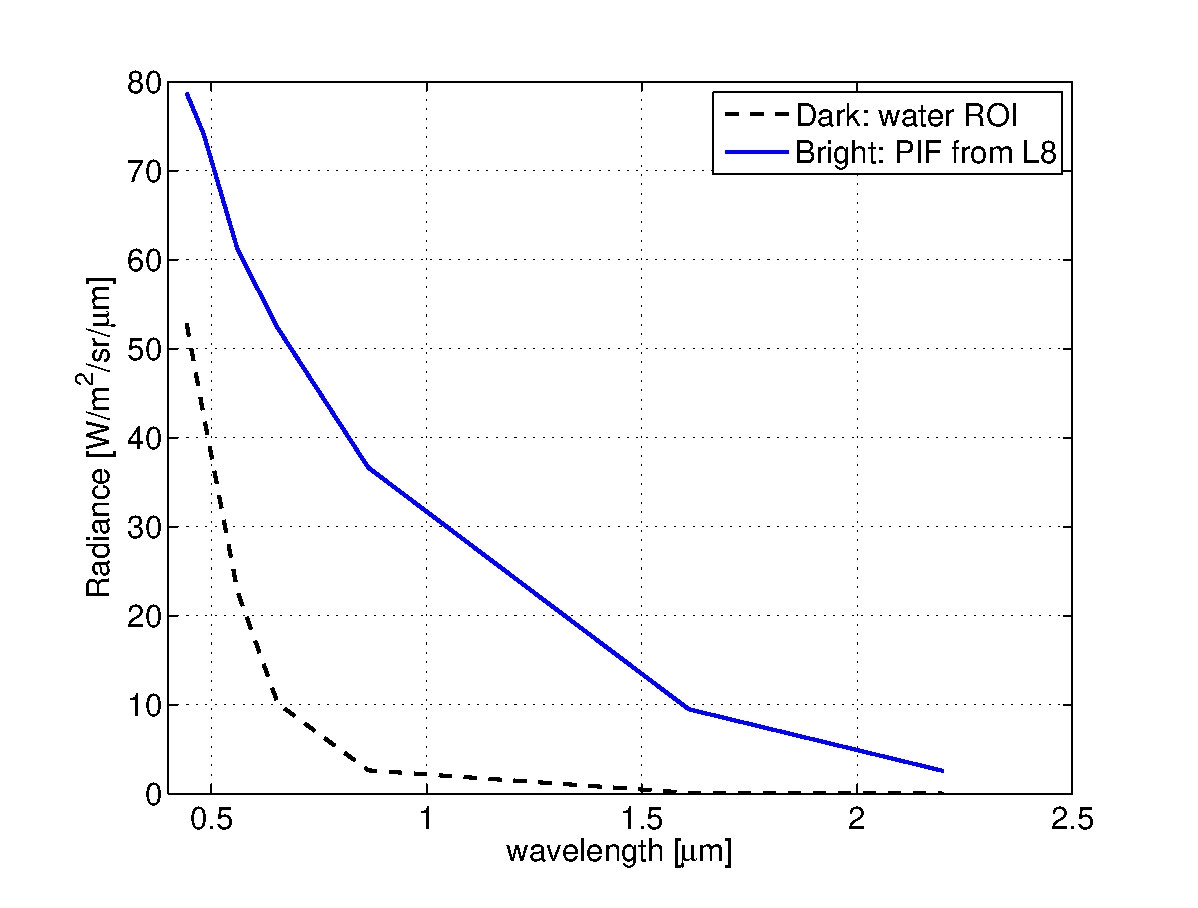
\includegraphics[width=8cm]{./Images/ELMrad130929_150422}
    % \vspace{1.5cm}
    \centerline{(a)}\medskip
  \end{minipage}
  \hfill
  \begin{minipage}[d]{0.48\linewidth}
    \centering
      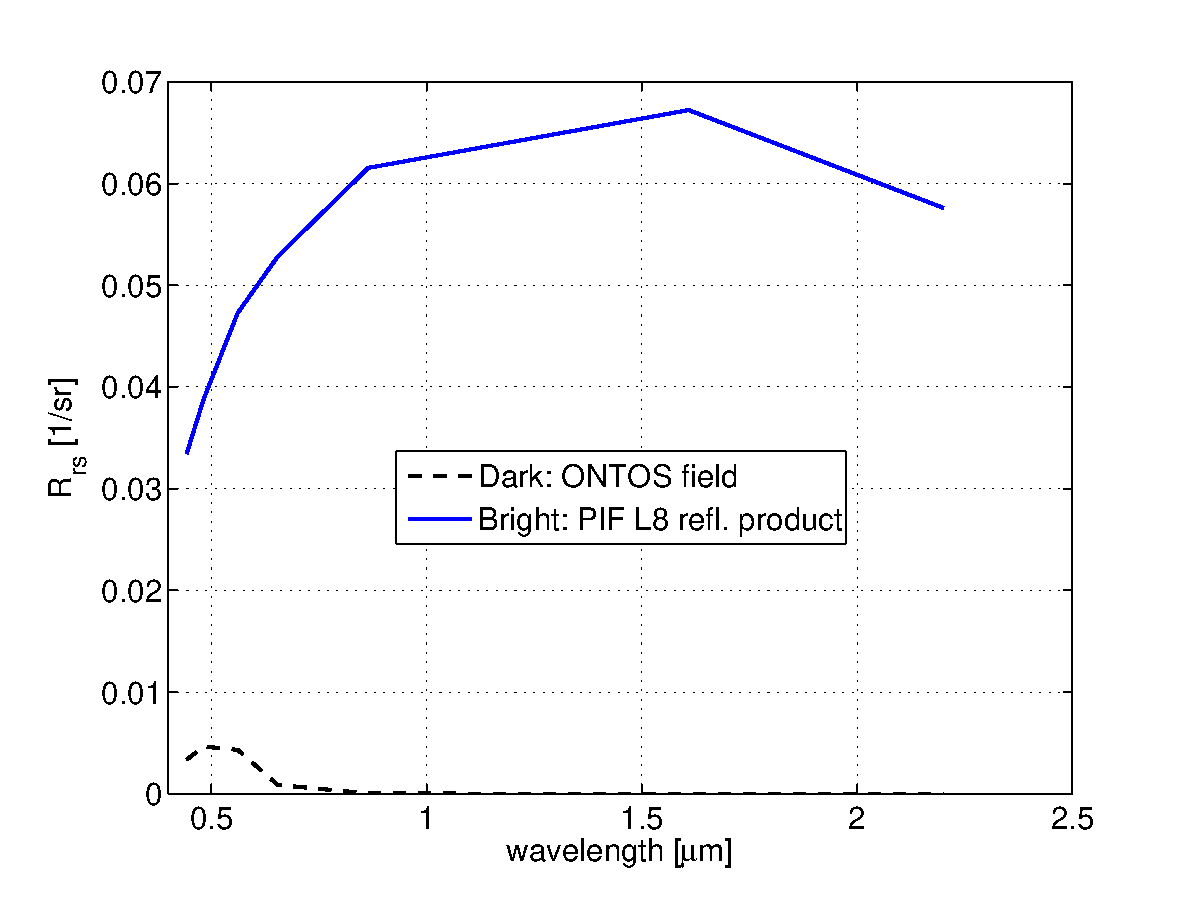
\includegraphics[width=8cm]{./Images/ELMRrs130929_150422}
    % \vspace{1.5cm}
    \centerline{(b)}\medskip
  \end{minipage}
  \caption{Example of the bright and dark pixel used in the MoB-ELM atmospheric correction method for Landsat 8 scene acquired on 09-19-2013.\label{fig:MOBELMpxls} } 
\end{figure}

% ---------------------------------------------------------------
\subsubsection{Black Pixel Determination}
\label{subsubsec:blackpixel}

The Landsat surface reflectance product cannot be used for the dark pixel target because the product is not precise enough over water. Therefore, the $R_{rs}$ spectra for the dark pixel target is obtained from the Ecolight model, which is a special version of the Hydrolight model that runs faster. The Hydrolight model is a radiative transfer numerical model that computes radiance distribution and derived quantities (e.g. $R_{rs}$) for natural water bodies (\cite{MobleyHE}). The view angle of interest for this work is only the nadir angle, and therefore, Ecolight is a more convenient option. It is suggested to use the Ecolight model when only the nadir-viewing $R_{rs}$ is needed since the Ecolight model only solves the azimuthal averaged version of the radiative transfer equation (RTE). Solving only the azimuthal average version of the RTE requires much less computer time than solving the RTE for all azimuthal directions to have the full radiance distribution as in Hydrolight (\cite{MobleyHE}). Note that Ecolight uses exactly the same inputs as Hydrolight.

The dark pixel is taken from a region of interest (ROI) over water present in the Landsat 8 radiance image with a low concentration of CPAs. Inherent optical properties (IOPs) and CPA concentration measurements taken in the field (or estimated from ancillary sources) for the same ROI are input to Ecolight. The field and lab measurements are described in the Results and Discussion section (Section \ref{sec:Results}) below. The ``Case 2 model'' in Ecolight is used to generate a $R_{rs}$ spectra for the dark pixel to be used in the MoB-ELM method. This Case 2 model is a generic four-component (pure water, chlorophyll-bearing particles, CDOM, and mineral particles) IOP model (\cite{MobleyHEtech}). Concentration, phase function, and mass-specific absorption and scattering coefficient spectra for each CPA need to be input separately in the Case 2 model of Ecolight. 

An example of the inputs used to generate the $R_{rs}$ spectra of the dark pixel for a particular date is specified below. \autoref{tab:ONTNSconc} shows the CPAs concentrations for two different water samples from the stations of the data collection on September, 19th, 2013. The location of these stations is shown in \autoref{fig:091913Sites}. These water samples were collected near the shore of Lake Ontario (labeled as ONTNS) and from the southern part of Long Pond (labeled as LONGS), and they represent two scenarios with totally different concentration of CPAs. The concentration of CPAs are chlorophyll-{\it a} concentration, $C_a$ $[mg~m^{-3}]$, total suspended solids concentration, $TSS$ $[g~m^{-3}]$ (a.k.a. suspended particulate matter (SPM) concentration or suspended minerals (SM)), and CDOM absorption coefficient at $\lambda_0=440nm$, $a_{CDOM}(\lambda_0=440nm)$ $[1/m]$. The water sample ONTNS was used to generate the reflectance spectra for the dark pixel in Ecolight since it exhibits a low concentration of CPAs. The concentrations for each component were set to be constant with depth in Ecolight with the values obtained from field measurements shown in \autoref{tab:ONTNSconc}.

\begin{table}[htbp!]
\caption{ CPA concentrations of the water samples collected for two stations on the 09-19-2013 collection (\autoref{fig:091913Sites}) used as input in Ecolight (Labels: ONTNS: Lake Ontario near-shore and LONGS: Long Pond south). \label{tab:ONTNSconc} } 
\small
\centering
\begin{tabular}{c|c|c|c} 
 Station & \bfseries{$C_a$} & \bfseries{$TSS$} & \bfseries{$a_{CDOM}(\lambda_0=440nm)$}\\
 & $[mg~m^{-3}]$ & $[g~m^{-3}]$ & $[1/m]$ \\ \hline \hline
ONTNS & 0.48   & 1.6  & 0.1151 \\ 
LONGS & 112.76 & 46.0 & 1.1953 \\ 
 \end{tabular}
\end{table}

\begin{figure}[htb]
  \centering
  \includegraphics[trim=0 90 0 110,clip,width=16cm]{./Images/ROI_RocEmbayment130919_150424}
  \caption{Landsat 8 scene acquired on 09-19-2013 (scene LC80160302013262LGN00) showing the sites in the Rochester Embayment for the water sample collection. (Labels: ONTNS: Lake Ontario near-shore, ONTOS: Lake Ontario off-shore, LONGS: Long Pond south, LONGN: Long Pond north, CRANB: Cranberry Pond and IBAYN: Irondequoit Bay north)\label{fig:091913Sites} } 
\end{figure}

\begin{figure}[htb]
  \centering
  \includegraphics[trim=0 50 0 110,clip,width=16cm]{./Images/ROI_RocEmbayment140929_150424}
  \caption{Landsat 8 scene over the Rochester Embayment for the water sample collection on 09-29-2014 (scene LC80170302014272LGN00).\label{fig:092914Sites} } 
\end{figure}

The absorption properties for the component chlorophyll-{\it a} were input by user-supplied data files containing mass-specific absorption coefficients as a function of wavelength. This mass-specific absorption spectra is shown in \autoref{fig:CHLcoef}.(a)\todo{typo in a* units!}. This data was obtained from lab measurements of absorption coefficient spectra for the water sample ONTNS with a spectrophotometric method following SeaWiFS protocols (\cite{Mueller1995}). The spectrophotometric method yields absorption coefficients, which are converted to mass-specific absorption coefficients by dividing the absorption coefficients spectra by its concentration ($C_a$). This $C_a$ was determined in lab by a spectrophotometric method as well. For the chlorophyll-{\it a} scattering properties, the same mass-specific scattering coefficient data used in \cite{Raqueno:2000} and \cite{Raqueno:2003} were utilized. These data were characterized through laboratory studies as part of a data collection on May 20, 1999 over the same area of study. These data are shown in \autoref{fig:CHLcoef}.(b). A Fournier-Forand (FF) phase function with a backscatter fraction of 0.010 was selected as the scattering phase function for chlorophyll-{\it a}. The details about the selection of this specific phase function will be described below.

\begin{figure}[htb]
  	\begin{minipage}[c]{0.48\linewidth}
    	\centering
  		\includegraphics[height=6cm]{./Images/CHLaastJavier.eps}
  		% \caption{Chlorophyll mass-specific absorption spectra used for the determination of the $R_{rs}$ spectra of the dark pixel in Ecolight. \label{fig:CHLaast} } 
		\centerline{(a)}\medskip
  	\end{minipage}  
  	\hfill
  	\begin{minipage}[c]{0.48\linewidth}
    	\centering
  		\includegraphics[height=6cm]{./Images/CHLbastRolo.eps}
  		% \caption{Chlorophyll mass-specific scattering spectra used for the determination of the $R_{rs}$ spectra of the dark pixel in Ecolight. \label{fig:CHLbast} } 
  		\centerline{(b)}\medskip
  	\end{minipage}	
  	\caption{Chlorophyll mass-specific absorption (a) and scattering (b)spectra used for the determination of the $R_{rs}$ spectra of the dark pixel in Ecolight. \label{fig:CHLcoef} } 
\end{figure}

For the CDOM component, the absorption specification $a_{CDOM}(\lambda)$ was input following the format required by Ecolight. First, the absorption coefficients were determined by spectrophotometric lab measurements for the ONTNS water sample. These data are shown in \autoref{fig:CDOMcoef}.(a). Then, the data were normalized by the absorption value $a(\lambda_0)=0.1151[1/m]$ at the reference wavelength $\lambda_0=440nm$, so that $a^*(\lambda_0)=1$. These normalized data are shown in \autoref{fig:CDOMcoef}.(b) as purple dots. An exponential curve with the following equation

\begin{equation}
	\label{eq:CDOMabs}
	a^*(\lambda)=a^*(\lambda_0)\exp{\left[-\gamma(\lambda-\lambda_0)\right]}
\end{equation}

\noindent was fitted to the normalized data. It was determined that the decay constant $\gamma=0.0126$. The fitted curve is illustrated in \autoref{fig:CDOMcoef}.(b) as a solid line. The parameters of this fitted curve are input into Ecolight to specify the CDOM normalized mass-specific absorption $a^*$, and $a(\lambda_0)=0.1151[1/m]$ to specify the CDOM absorption coefficient at the reference wavelength $\lambda_0=440nm$.

\begin{figure}[htbp!]
	\begin{minipage}[c]{0.48\linewidth}
  		\centering
  		\includegraphics[height=5.5cm]{./Images/ONTNS_CDOMabs.eps}
  		% \caption{CDOM absorption coefficient spectra used for the determination of the $R_{rs}$ spectra of the dark pixel in Ecolight. \label{fig:CDOMa} } 
		\centerline{(a)}\medskip
  	\end{minipage}  
  	\hfill
  	\begin{minipage}[c]{0.48\linewidth}
    	\centering
  		\includegraphics[height=5.5cm]{./Images/ONTNS_CDOMfitting.eps}
  		% \caption{CDOM mass-specific absorption spectra used for the determination of the $R_{rs}$ spectra of the dark pixel in Ecolight. \label{fig:CDOMaast} }
  		\centerline{(b)}\medskip
  	\end{minipage}  
  	\caption{CDOM absorption (a) and mass-specific absorption (b) coefficient spectra used for the determination of the $R_{rs}$ spectra of the dark pixel in Ecolight. \label{fig:CDOMcoef} }
\end{figure}

The mineral mass-specific absorption coefficient was determined in the same fashion as for the chlorophyll mass-specific absorption coefficient from lab measurements of the ONTNS water sample. The mineral mass-specific absorption coefficients are shown in \autoref{fig:SMcoef}.(a). The mineral mass-specific scattering coefficients are the same used by \cite{Raqueno:2000} and \cite{Raqueno:2003} and are shown in \autoref{fig:SMcoef}.(b). An FF phase function with backscatter fraction 0.010 was selected as the scattering phase function for the minerals. The details about the selection of this specific phase function will be described below.

\begin{figure}[htbp!]
	\begin{minipage}[c]{0.48\linewidth}
  		\centering
  		\includegraphics[height=5.5cm]{./Images/SMaastJavier.eps}
  		% \caption{Mineral mass-specific absorption spectra used for the determination of the $R_{rs}$ spectra of the dark pixel in Ecolight. \label{fig:SMaast} } 
	  	\centerline{(a)}\medskip
  	\end{minipage}  
  	\hfill
  	\begin{minipage}[c]{0.48\linewidth}
  		\centering
  		\includegraphics[height=5.5cm]{./Images/SMbastRolo.eps}
  		% \caption{Mineral mass-specific scattering spectra used for the determination of the $R_{rs}$ spectra of the dark pixel in HydroLight. \label{fig:SMbast} } 
  		\centerline{(b)}\medskip
  	\end{minipage}
  	\caption{Mineral mass-specific absorption (a) and scattering (b) coefficient spectra used for the determination of the $R_{rs}$ spectra of the dark pixel in Ecolight. \label{fig:SMcoef} }
\end{figure}

The following parameters were input to Ecolight in order to simulate the Landsat 8 acquisition conditions. The illumination conditions were input to Ecolight by specifying the solar zenith angle and day of the year that matched the Landsat 8 image. Internal sources and inelastic scatter were not included in the simulations, as we did not have this information. The wavelength range was $[400nm,1000nm]$, with a $1nm$ step. Default values for the air-water surface conditions were used, with a windspeed equal to $5m/s$, a real index of refraction equal to $n=1.34$, and the semi-empirical sky model (based on RADTRAN-X). Recall that Hydrolight uses a Cox-Munk air-water surface model that parameterizes gravity and capillary waves via the wind speed (\cite{MobleyHEtech}). Finally, the bottom boundary condition used in Ecolight was ``the water column is infinitely deep.''

One of the input parameters needed by Ecolight is the scattering phase function for each component. Ecolight generates a Fournier-Forand phase function for a given backscatter fraction, $b_b/b$, where $b$ is the total scattering coefficient (for all directions) and $b_b$ is the scattering coefficient only in the backward direction. By default in Ecolight, $b_b/b$ could have values between $0.0001$ and $0.50$ (i.e. [$0.01\%$-$50\%$]). There was no empirical information available about $b_b/b$ so the following approach was used to determine the scattering phase function for both the chlorophyll-{\it a} and the mineral particle components. A LUT of $R_{rs}$ with different scattering phase functions was created in the following fashion: one Ecolight run was obtained for each discretized Fournier-Forand phase functions from the library of phase functions supplied with Ecolight 5.2, but maintained the rest of the input parameters to Ecolight the same, i.e. concentrations, IOPs, surface and bottom boundary conditions, atmospheric conditions, and geometry. These parameters correspond to the ONTNS water sample described above. The different $R_{rs}$ spectra in the LUT were compared with the $R_{rs}$ for ONTNS measured {\it in situ}. The best match was determining by choosing the lowest root mean squared error (RMSE) between the $R_{rs}$ for the ONTNS water sample measured {\it in situ} and the simulated $R_{rs}$ spectra for the ONTNS water sample. It was determined that the best match corresponds to the $R_{rs}$ in the LUT generated with a discretized Fournier-Forand phase function with a backscatter equal to $0.010$, i.e. $1\%$ of backscatter fraction (file name: FFbb010.dpf). 

The best match from the LUT of $R_{rs}$ with different phase functions was used as the $R_{rs}$ spectra of the dark pixel in the MoB-ELM method. This $R_{rs}$ is further spectrally sampled to the Landsat 8 spectral response. \autoref{fig:MOBELMpxls}.(b)\todo{change ONTOS to ONTNS in fig.}~ shows this $R_{rs}$ spectra as a black dashed line. Using a $R_{rs}$ generated in Hydrolight (i.e. a model-based dark pixel) instead of an {\it in situ} dark target in the MoB-ELM helps account for differences between atmospheric correction and the Hydrolight-based LUT used for retrieving the CPA concentrations (explained in the following Section \ref{subsec:LUT}).

The radiance spectra for the dark pixel is obtained from an ROI in the Landsat 8 radiance image that includes the ONTNS station. Statistics are computed in this dark region, and the mean values in each band is used as the radiance spectra for the dark pixel. This radiance spectra for the dark pixel is shown in \autoref{fig:MOBELMpxls}.(a) as a black dashed line.

As a review, \autoref{fig:MOBELMpxls} shows the different spectra used to perform the MoB-ELM atmospheric correction method, where four different spectra can be seen: one $R_{rs}$ and one radiance spectra for the bright pixel (obtained using the PIF extraction over the Provisional Landsat 8 Surface Reflectance product and Landsat 8 image, respectively), one $R_{rs}$ spectra for the dark pixel (obtained from HydroLight), and one radiance spectra for the dark pixel (obtained from the statistics of a ROI over water in the Landsat 8 image). These spectra are used by the MoB-ELM to atmospherically correct the Landsat 8 image using the ENVI Classic software (\cite{ENVIUserGuide}). This is performed using the ``Empirical Line'' algorithm of the ``Calibration Utilities'' in ENVI classic, where the Landsat 8 image is used as the input image, and the $R_{rs}$ spectra are labeled as ``field spectra'' and the radiance spectra are labeled as ``data spectra.'' The final product of this process is an image in $R_{rs}$ values for each water pixel, which will be used to perform the retrieval of CPAs concentrations described in Section \ref{subsec:Retrieval} below. 

\todo{include summary of MoB-ELM} 
% ---------------------------------------------------------------
\subsection{LUT Generation}
\label{subsec:LUT}
A LUT of $R_{rs}$ is generated in Ecolight for different combinations of CPA concentrations and scattering phase functions. \autoref{tab:LUTconc2} shows the different parameters used to create the LUT in Ecolight. Ecolight was used in the same fashion as in the black pixel determination for the MoB-ELM (Section \ref{subsubsec:blackpixel}). Two different sets of IOPs (mass-specific absorption and scattering spectra) were used, one set for modeling the open lake conditions (low concentration of CPAs) from the lab measurements for the ONTNS site, and one set for modeling the ponds condition (high concentration of CPAs) from the lab measurements for the LONGS site\todo{show IOPs figures}. These IOPs are labeled in \autoref{tab:LUTconc2} as ``ONTNS'' for the open lake conditions and as ``LONGS'' for the ponds' conditions. \autoref{tab:LUTconc2} also shows the CPAs concentration used to create the LUT in Ecolight. Furthermore, different discretized Fournier-Forand phase functions with four different $b_b/b$ values (i.e. $0.5$, $1.0$, $1.5$ and $2.0\%$) were used for the Chlorophyll-{\it a} and mineral particles scattering phase functions.

\begin{table}[htb]
\caption{Input parameters for the LUT generation in Ecolight for the Landsat 8 image acquired on 09-19-2013. \label{tab:LUTconc2}} 
\small
\centering
		\begin{tabular}{c|c|c|c|c}
		\hline \hline
        		IOPs Input & \bfseries{$C_a$} & \bfseries{$TSS$} & \bfseries{$a_{CDOM}(440nm)$} & \bfseries{$b_b/b$}   	\\
				           & $[mg~m^{-3}]$			  & $[g~m^{-3}]$ 			 & 	$[1/m]$ 					& $[\%]$		  	  	\\ \hline \hline
ONTNS 	&  0.1  	& 1.0  		&  0.11		&  0.3 	\\
-- 		&  0.5  	& 2.0  		&  0.15		&  0.4 	\\
--    	&  1.0  	& 5.0  		&  0.21		&  0.5 	\\
--    	&  3.0  	& 10.0		&  0.6 		&  0.6 	\\ 
-- 		&  10.0     & -- 		&  --		&  0.7	\\	
--    	&  20.0     & -- 		&  --		&  1.0	\\	
--    	&  40.0     & -- 		&  --		&  1.4	\\
--    	&  --       & -- 		&  --		&  2.0	\\ \hline

LONGS 	&  60.0  	& 25.0		&  1.0 		&  0.3  \\
--    	&  90.0  	& 45.0		&  1.2 		&  0.4  \\
--    	&  110.0 	& 50.0		&  --  		&  0.5  \\
--    	&  --   	& --    	&  --  		&  0.6  \\  
--    	&  --   	& --   		&  --  		&  0.7 	\\  
--    	&  --   	& --   		&  --  		&  1.0 	\\   
--    	&  --   	& --   		&  --  		&  1.4 	\\  
--    	&  --   	& --   		&  --  		&  2.0 	\\  \hline \hline
% --    	&  135.0	& --   		&  --  		&  --  	\\  
% --    	&  150.0	& --   		&  --  		&  --  	\\ \hline 
	 	\end{tabular}
	\end{table}

Then, the LUT of $R_{rs}$ obtained from Ecolight is spectrally sampled to the OLI's spectral response. As an example, the LUT created with the parameters shown in \autoref{tab:LUTconc2} in Ecolight for the Landsat 8 image acquired on 09-19-2013 is shown in \autoref{fig:LUT}. This particular LUT has $1170$ elements spectrally sampled to the OLI's spectral response\todo{Checked until here!}.

\begin{figure}[htb]
    \centering
      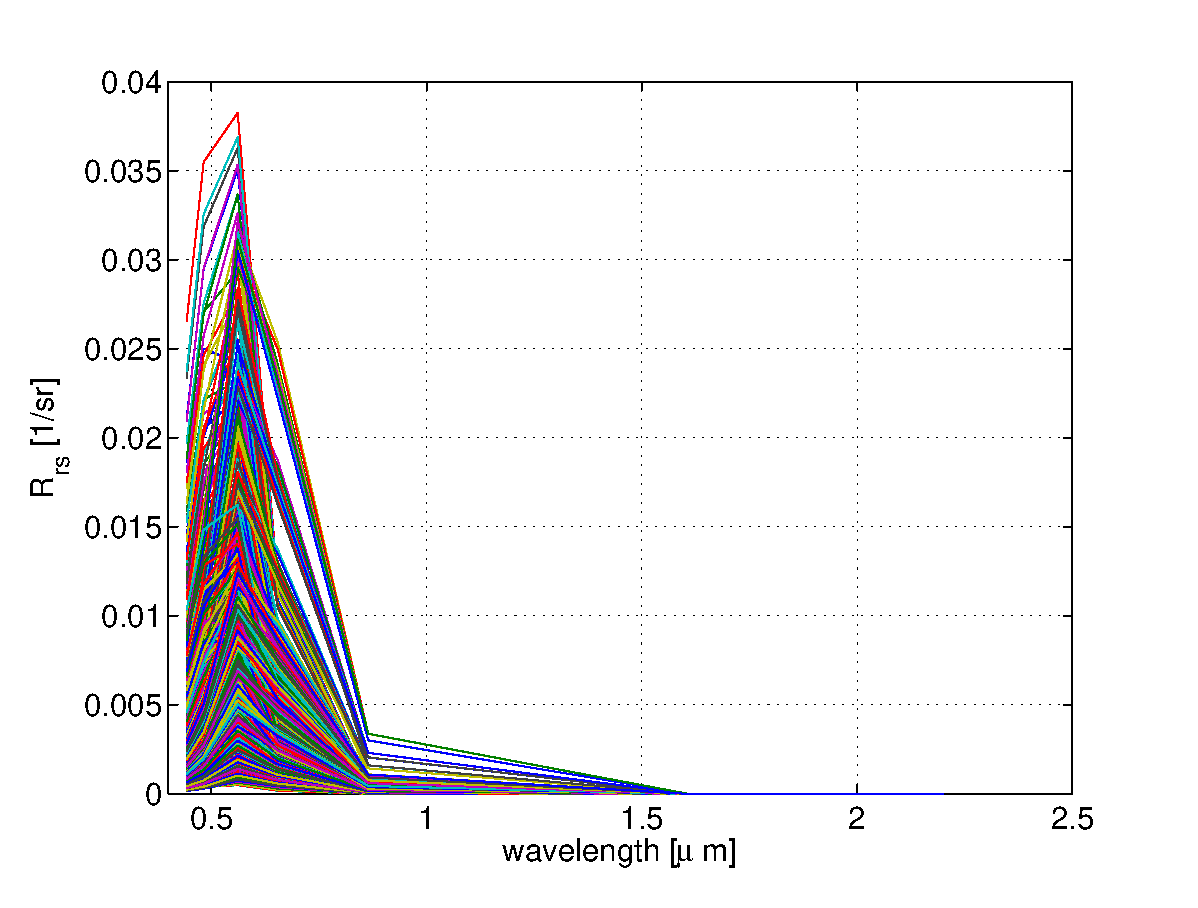
\includegraphics[height=6cm]{./Images/LUTsmart130919_150422.eps}
      \caption{LUT with $1170$ elements created in Ecolight for the Landsat 8 scene acquired on 09-19-2013. Each element was created from a combination of parameters in \autoref{tab:LUTconc2}.}
      \label{fig:LUT}
\end{figure}

% ============================================================
\subsection{Retrieval Algorithm} 
\label{subsec:Retrieval}
The retrieval of CPAs concentrations is based in the work done by \cite*{Gerace:2013}. A spectral-matching technique was applied with the purpose of finding the closest match to a given water $R_{rs}$ spectra within the LUT of $R_{rs}$ from Ecolight. In this work, the spectral matching was performed by minimizing the root mean squared error (RMSE), which is defined as

\begin{equation}
  RMSE(i) = \sqrt{\frac{1}{M}\sum_{m=1}^M\left[\widetilde{R}_{rs}(i,\lambda_m)-R_{rs}(\lambda_m)\right]^2}
\end{equation}

\noindent where $\widetilde{R}_{rs}(i,\lambda_m)$ is the $i$th $R_{rs}$ spectrum from the LUT at wavelength band $m$ and $R_{rs}(\lambda_m)$ is the water $R_{rs}$ spectrum at wavelength band $m$ from the atmospherically corrected Landsat 8 image. For each water pixel in the atmospherically corrected Landsat 8 image, the RMSE value is calculated for every $i$th element in the LUT. Then, the element of the LUT that results in the smallest RMSE value is chosen as the CPA concentrations for that particular water pixel. This method gives discretized values for the concentrations equal to the values used to create the LUT. The output is a concentration mapping for each CPA.
% % ============================================================
% \subsection{Ground Truth Data Collection and Lab Measurements}
% \label{subsec:FieldLabMea}
%%%%%%%%%%%%%%%%%%% SECTION %%%%%%%%%%%%%%%%%%%%%%%%%%%%%%%%
\section{Results and Discussion}
\label{sec:Results}
Field measurements were collected to support this study. Water samples were collected for each site in dark Nalgene bottles. Additionally, $R_{rs}$ spectra were measured using an ASD and a SVC instrument\todo{add citation for instruments}. Location for each site was recorded using a GPS. After collection, these water samples were analyzed in the lab at the Rochester Institute of Technology (RIT), and concentration and IOPs for each CPA were measured following the procedures described by \cite{Mueller1995}. These measurements are utilized as input to Ecolight for the LUT generation of the retrieval process and the black pixel determination for the MoB-ELM atmospheric correction algorithm. Also, some are utilized for validation of the retrieval process. The $C_a$ and $TSS$ measurements were validated by comparing with measurements analyzed by a credible lab (Monroe County Environmental Laboratory). This comparison between labs showed agreement in the measurements.

The MoB-ELM atmospheric correction algorithm discussed above was applied to the Landsat 8 scene collected on 09-19-2013 (scene LC80160302013262LGN00) over the Rochester Embayment (latitude: $43^\circ15'32.5''$N and longitude: $77^\circ36'13.1''$W) shown in \autoref{fig:L8Image130919}, \autoref{fig:091913Sites} and \autoref{fig:092914Sites}. This area of study was chosen because it included different water bodies with a wide range of CPAs characteristics, which helps to test the retrieval algorithm over unlike scenarios. These water bodies include ponds (Long Pond and Cranberry Pond) with high concentration of CPAs and Lake Ontario with low concentration of CPAs. As an example of the MoB-ELM results, \autoref{fig:RrsROIs130919} shows the $R_{rs}$ spectrum for four different stations of the 09-19-2013 Landsat 8 scene (\autoref{fig:091913Sites}). The shape of these spectra resemble $R_{rs}$ of water pixels. Also, the spectrum corresponding to low concentration of CPAs (i.e. ONTOS: Lake Ontario off-shore and ONTNS: Lake Ontario near-shore) can be distinguished from the rest of the spectrum corresponding to higher concentration of CPAs (i.e. LONGS: Long Pond south, CRANB: Cranberry Pond).

\begin{figure}[htbp!]
  \centering
  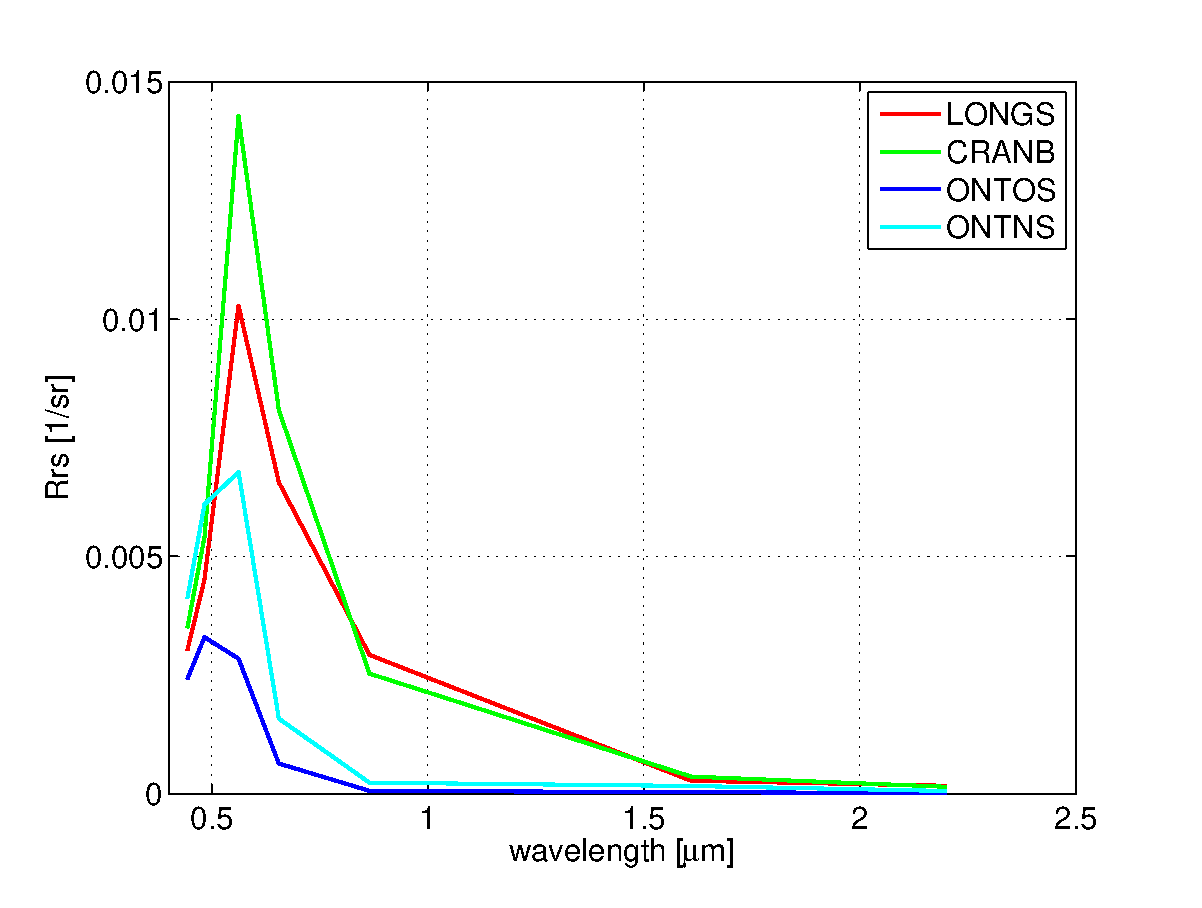
\includegraphics[height=6cm]{./Images/ROI130919_150422}
  \caption{$R_{rs}$ for the sites for the 09-19-2013 collection after applying the MoB-ELM atmospheric correction (Labels: LONGS: Long Pond south, CRANB: Cranberry Pond, ONTOS: Lake Ontario off-shore, and ONTNS: Lake Ontario near-shore).\label{fig:RrsROIs130919} } 
\end{figure}

After atmospherically correcting the Landsat 8 image, the retrieval of CPAs algorithm is applied to the area of study. The results of the retrieval for the 09-19-2013 scene is illustrated in the left-hand side of \autoref{fig:CPAsMaps130919} as a concentration map for each CPA. These maps exhibit the expected trend of low concentrations in the lake and higher concentrations in the ponds. The right-hand side of \autoref{fig:CPAsMaps130919} shows a comparison between measured concentration from the field and retrieved concentration obtained from the retrieval for each CPA for the different sites in the area of study. The dashed line represent the 1:1 line. 

\begin{figure}[htbp!]
  \begin{minipage}[c]{0.55\linewidth}
  		\centering
      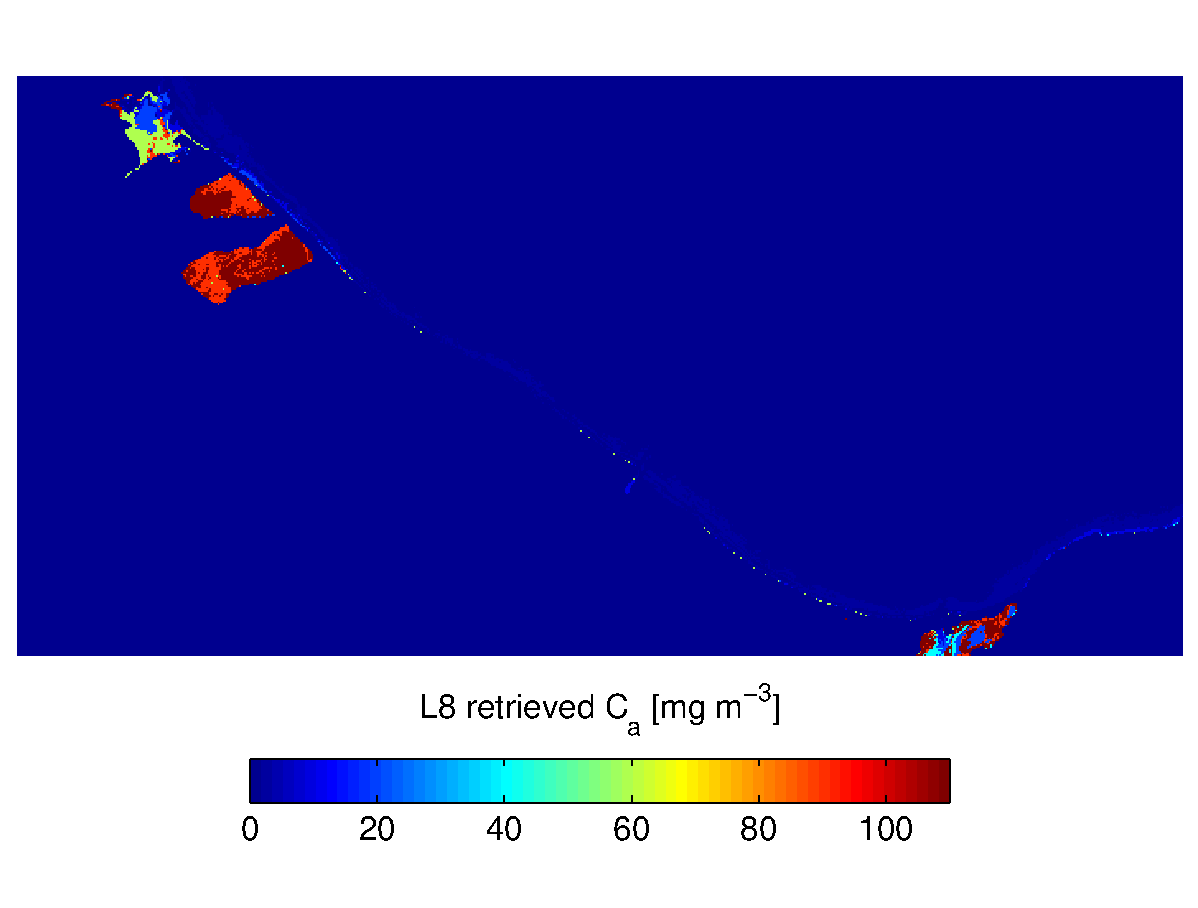
\includegraphics[trim=0 20 0 30,clip,height=6.8cm]{./Images/CHLmap130919_150420}  
  \end{minipage}
  \hfill
  \begin{minipage}[d]{0.35\linewidth}
      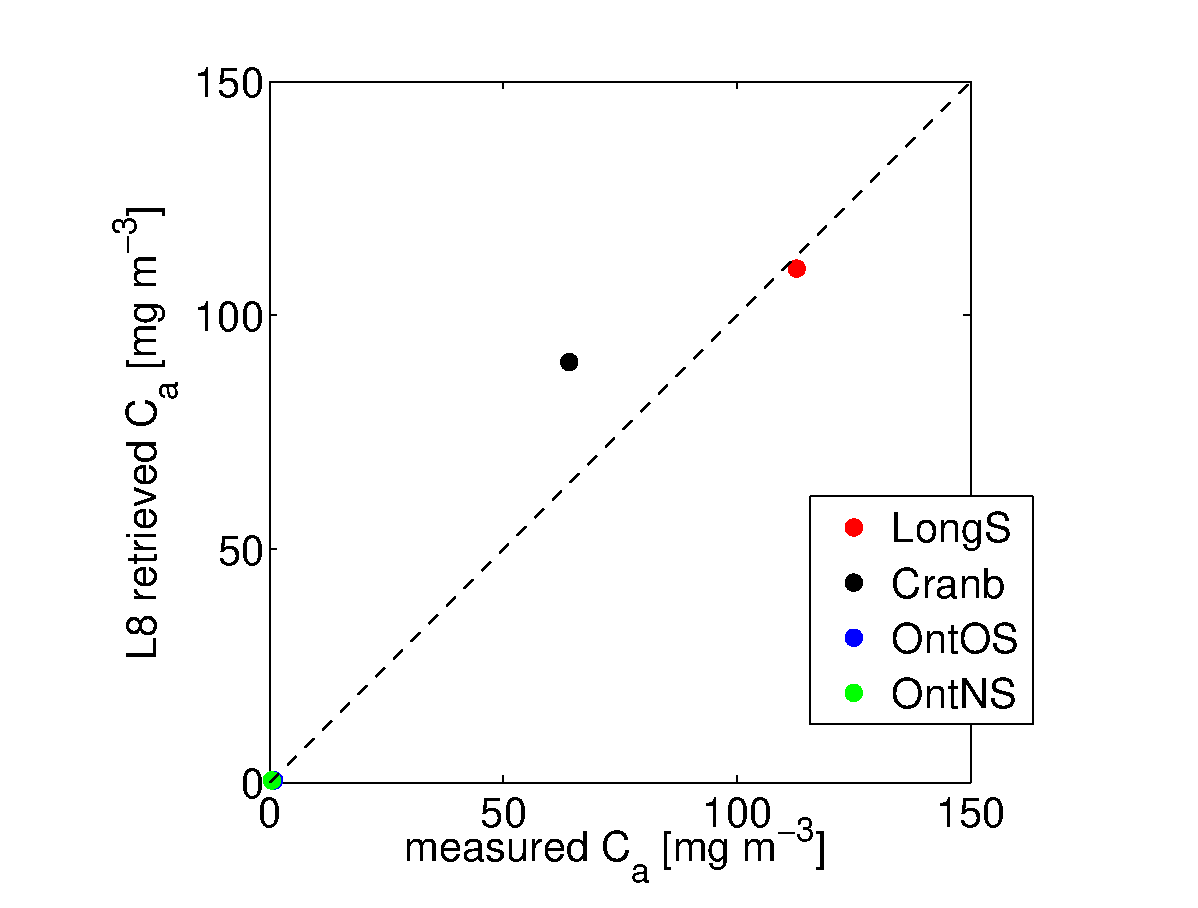
\includegraphics[trim=40 0 0 20,clip,height=5.5cm]{./Images/CHLretvsmea130919_150420}
  \end{minipage}
% 
%% TSS
  \begin{minipage}[c]{0.55\linewidth}
  		\centering
      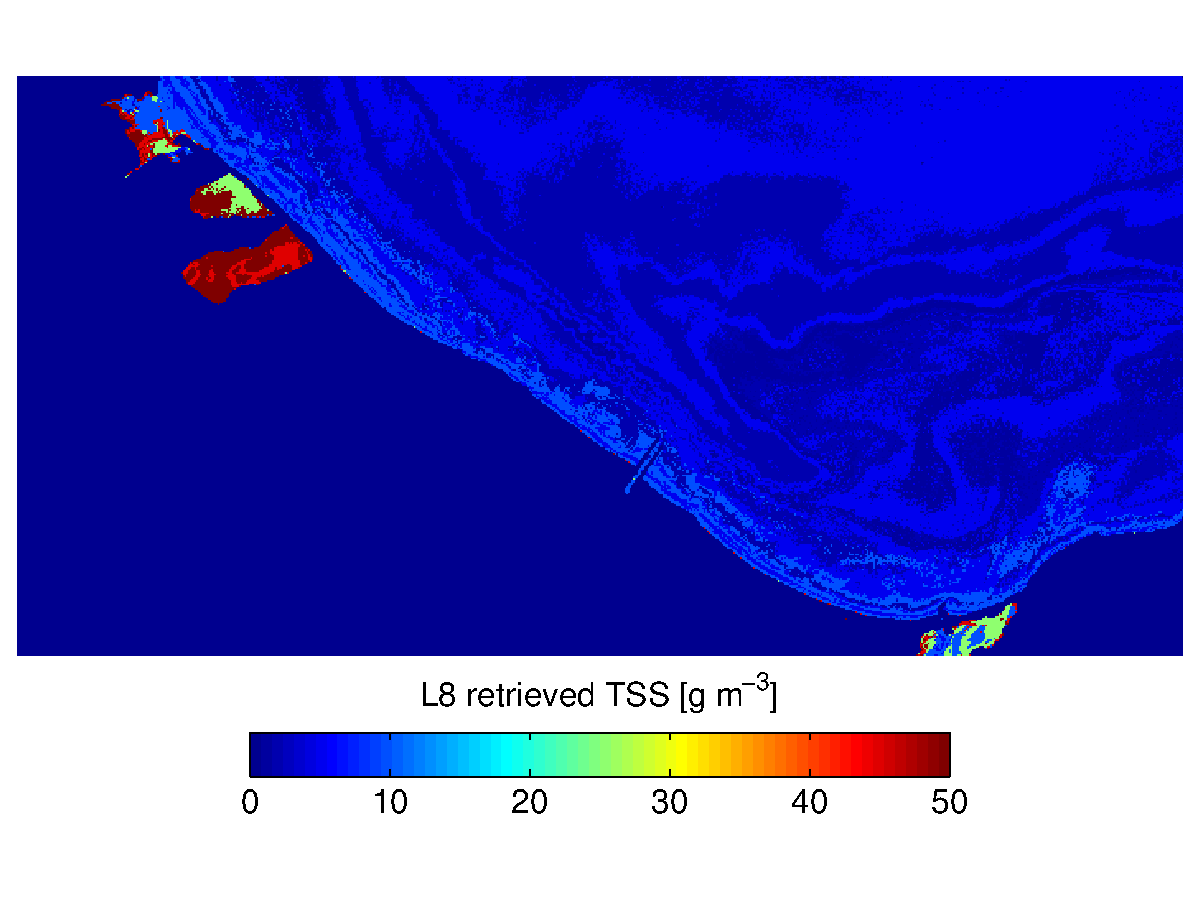
\includegraphics[trim=0 30 0 10,clip,height=6.8cm]{./Images/TSSmap130919_150420}  
  \end{minipage}
  \hfill
  \begin{minipage}[d]{0.35\linewidth}
      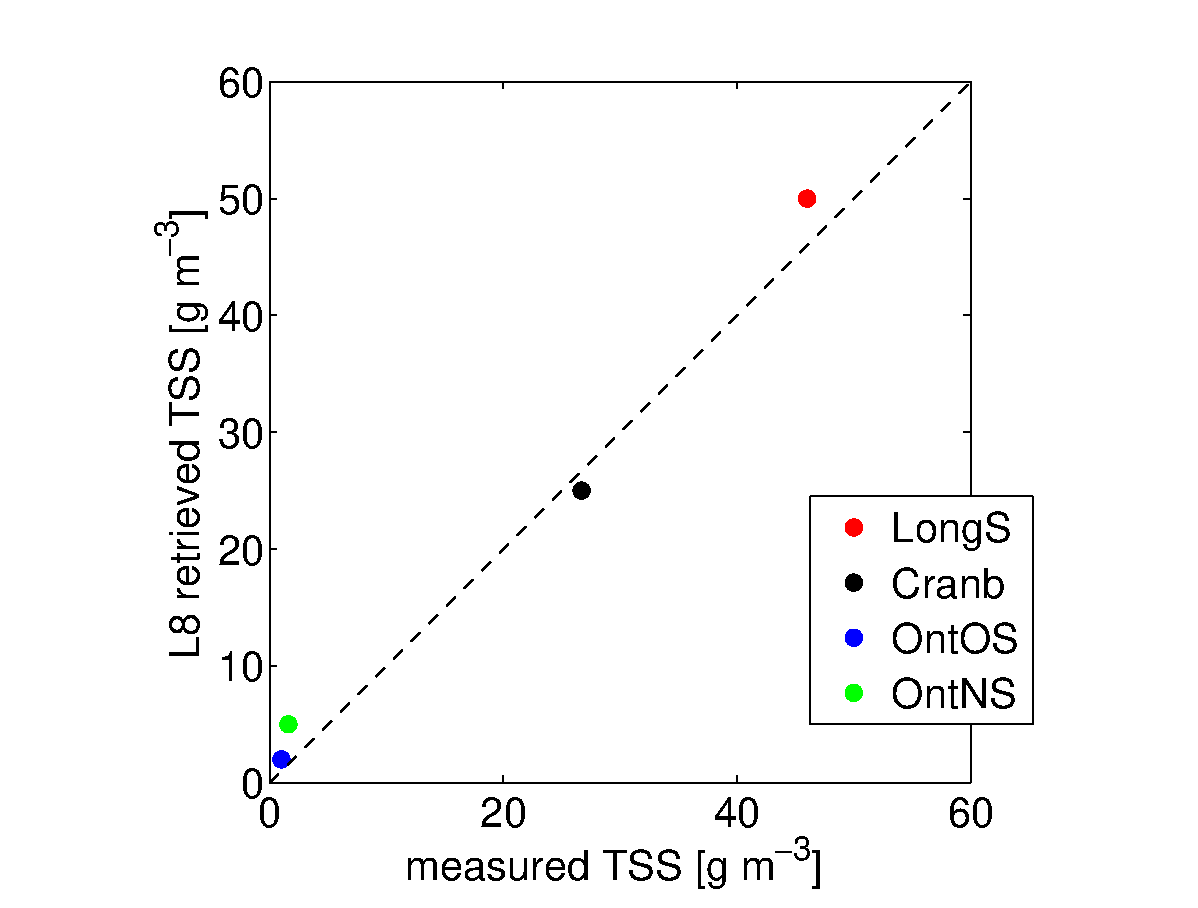
\includegraphics[trim=40 0 0 0,clip,height=5.5cm]{./Images/TSSretvsmea130919_150420}
  \end{minipage}

%% CDOM
  \begin{minipage}[c]{0.55\linewidth}
  		\centering
      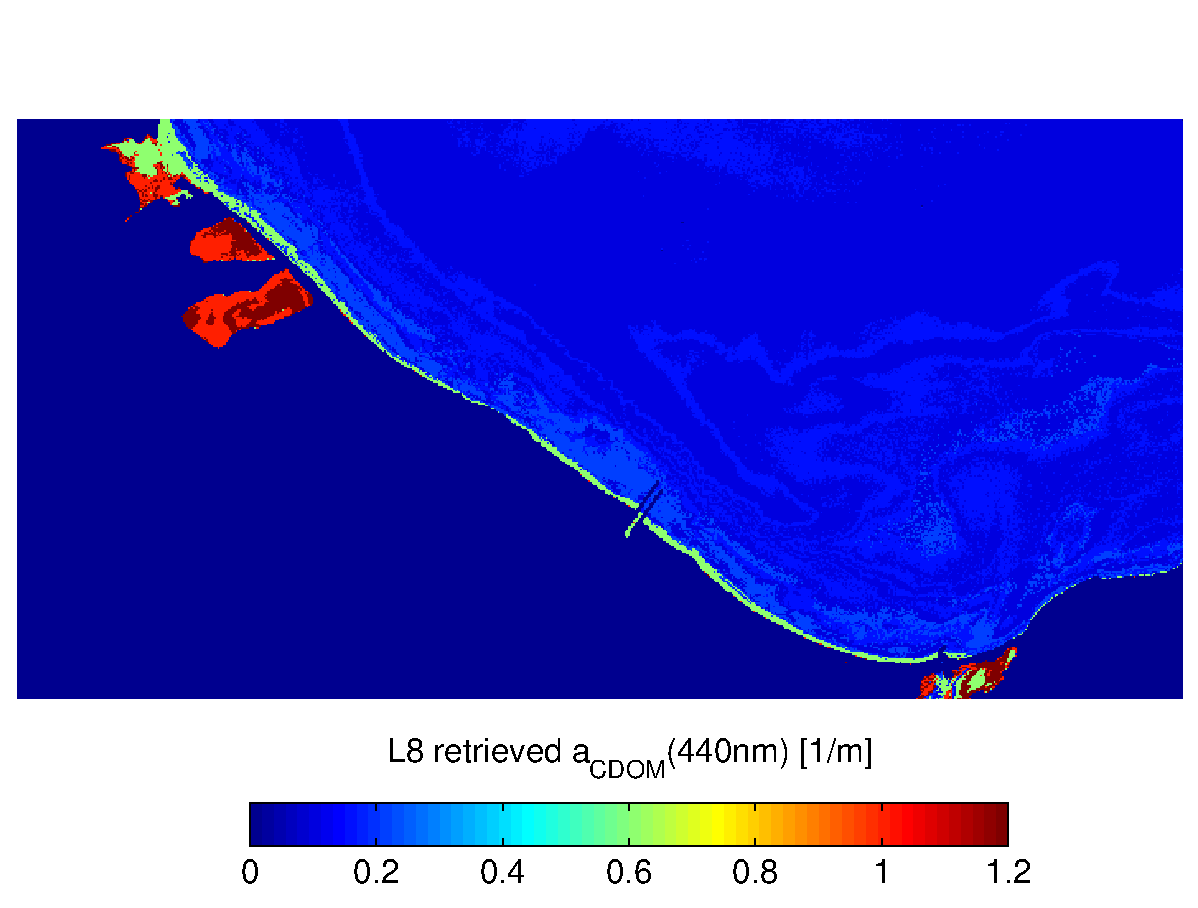
\includegraphics[trim=0 0 0 30,clip,height=6.8cm]{./Images/CDOMmap130919_150420}  
  \end{minipage}
  \hfill
  \begin{minipage}[d]{0.35\linewidth}
      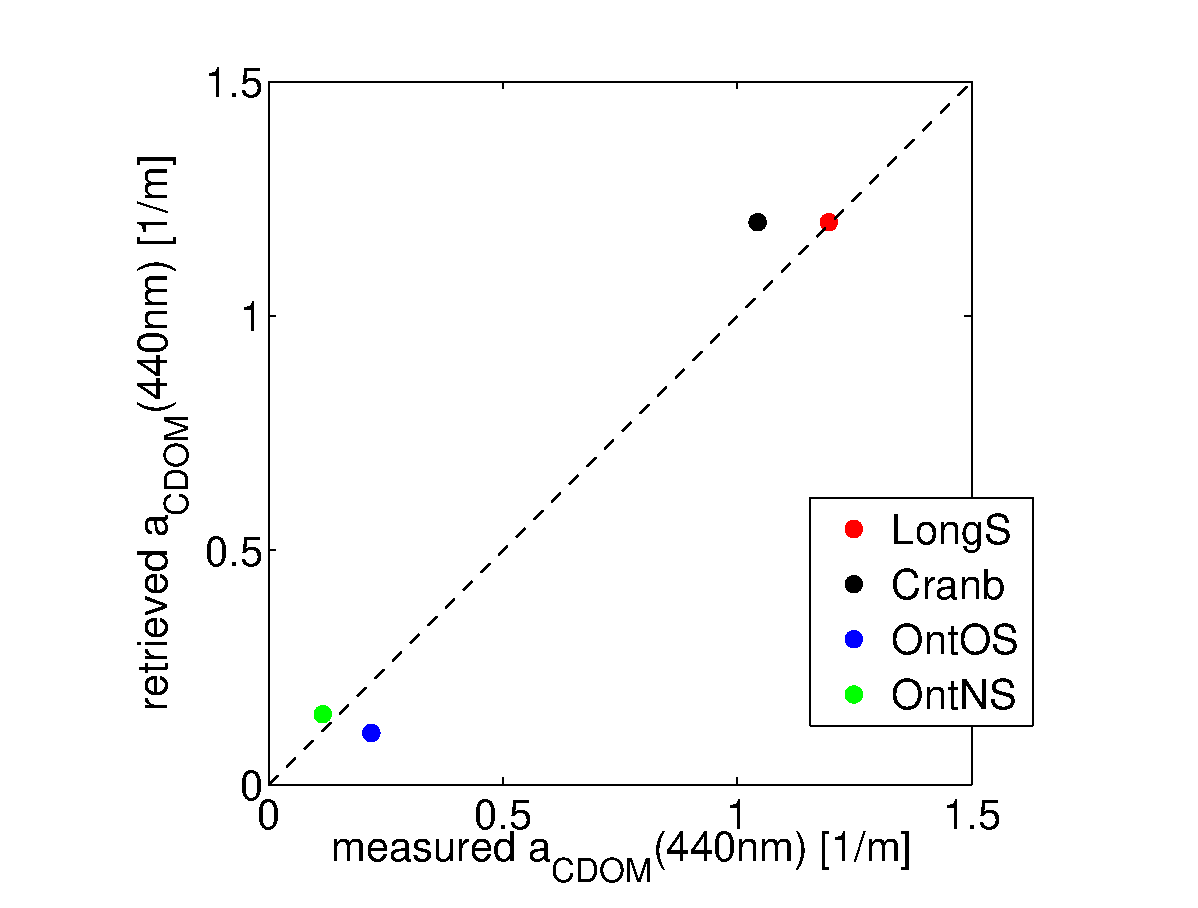
\includegraphics[trim=40 0 0 0,clip,height=5.5cm]{./Images/CDOMretvsmea130919_150420}
  \end{minipage}
% 
  \caption{CPA retrieval results for the Landsat 8 image acquired on 09-19-2013 (scene LC80160302013262LGN00). Concentration maps (left) and measured vs retrieved plots (right). The dashed line represent the 1:1 line. (Labels: LongS: Long Pond south, Cranb: Cranberry Pond, OntOS: Lake Ontario off-shore, and OntNS: Lake Ontario near-shore). \label{fig:CPAsMaps130919} } 
\end{figure}

% Preliminary results for concentration maps for each CPA over the Rochester Embayment, Rochester, NY are shown in \autoref{fig:CPAsMaps}  The expected trend of having low concentration of CPAs in the offshore of Lake Ontario and higher concentrations in the nearby ponds (Long Pond and Cranberry Pond) can be seen. 

% Comparisons between retrieved CPAs concentrations and field measurements are shown in \autoref{fig:CPAsMaps} for four different stations in the area of study. This comparison with field measurements showed good agreement at low concentrations but differences at higher concentrations. Ongoing work is focusing on incorporation of the IOP differences between water bodies in the LUT optimization process.
% Landsat 8 images from this area of study and corresponding water samples collected at the time of the satellite's overpass will be used to test the retrieval algorithm. So far, there are only three satisfactory images available from the summer 2013. This project contemplates performing one new ground truth data collection during 2014. Therefore, images from the 2013-2014 spring and summer collection seasons will be used to test the methodology. Note that a difficult challenge of this research is to obtain images with relatively clear weather conditions (i.e. cloud free) over the area of study.

% \autoref{fig:091913Sites} shows an image over this area of study for the data collection done on September, $19^{th}$, 2013  with the different sites as an example. The data collections are divided in two crews. One crew, named ``Lake crew'', is in charge of the Irondequoit Bay, Ontario near shore, Ontario off shore, Genesee River plume, Genesee River pier sites (labeled in \autoref{fig:091913Sites} as IBayN, OntNS, OntOS, RvrPLM and RvrPIER, respectively). The other crew, named ``Ponds crew'', is in charge of the Long Pond north and south, Cranberry Pond sites (labeled in \autoref{fig:091913Sites} as LongN, LongS and Cranb, respectively).
%% CHL

%%%%%%%%%%%%%%%%%%%%%%%%%%%%%%%%%%%%%%%%%%%%%%%%%%%%%%%%%%%%%%
\begin{figure}[htbp!]
  \begin{minipage}[c]{1.0\linewidth}
  		\centering
      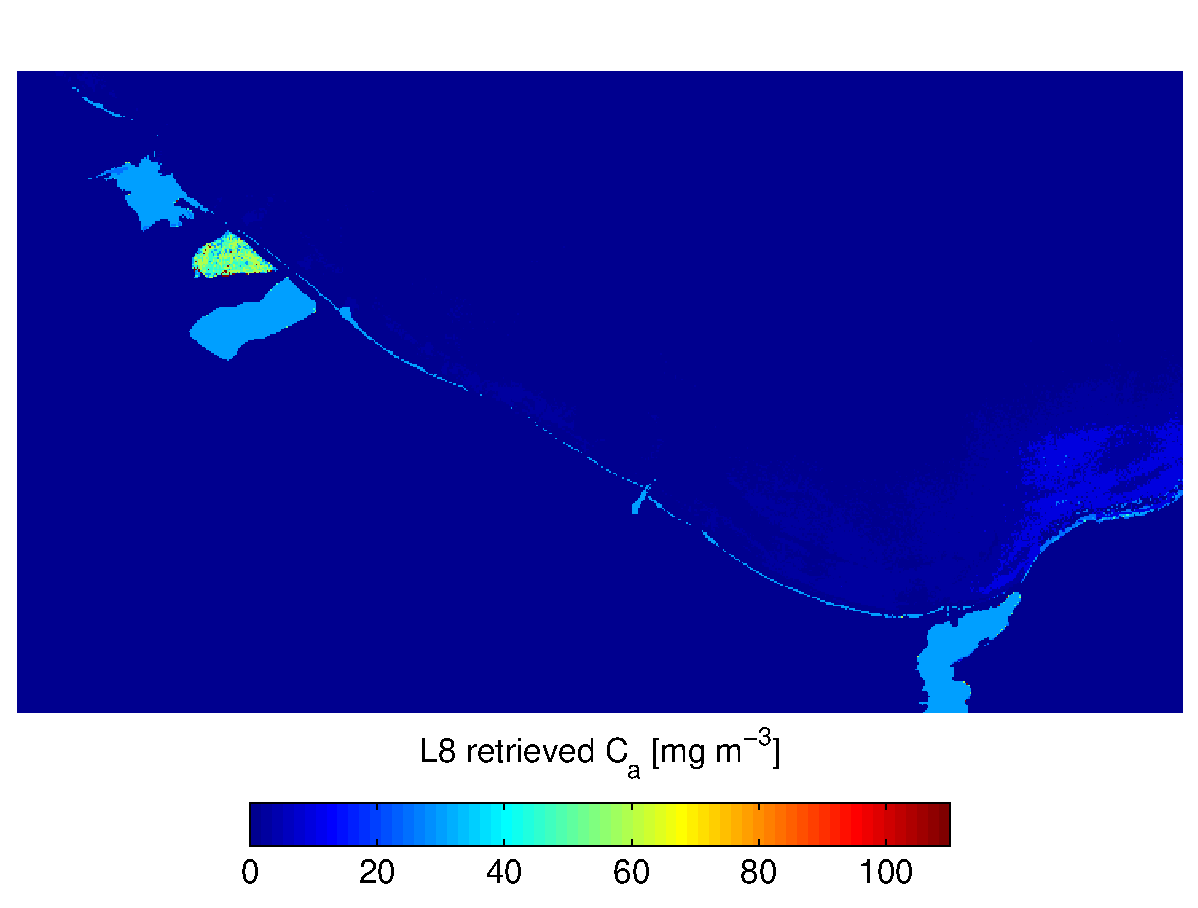
\includegraphics[trim=0 0 0 30,clip,height=7cm]{./Images/CHLmap140929_150420}  
  \end{minipage}\\
  % \hfill
  % \begin{minipage}[d]{0.45\linewidth}
      % 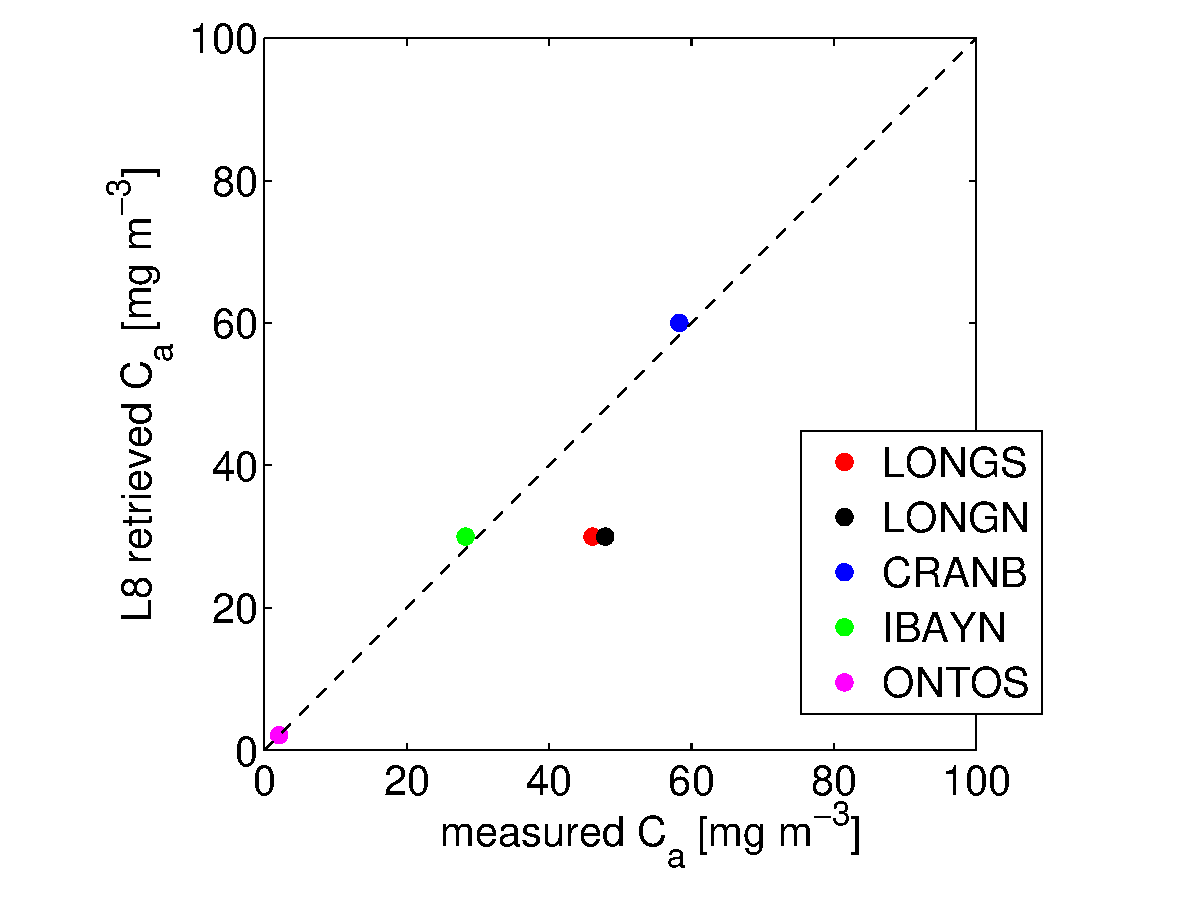
\includegraphics[height=5.5cm]{./Images/CHLretvsmea140929_150420}
  % \end{minipage}

%% TSS
  \begin{minipage}[c]{1.0\linewidth}
  		\centering
      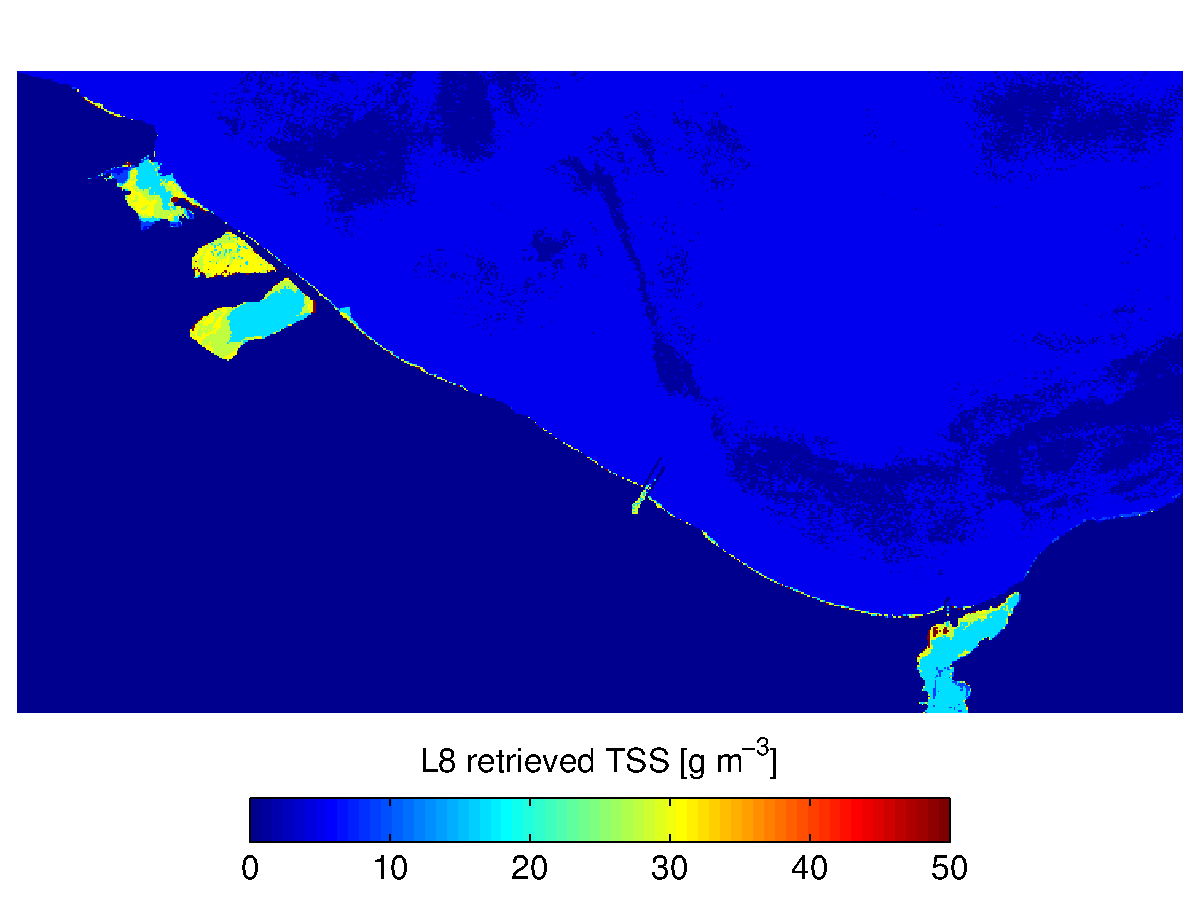
\includegraphics[trim=0 0 0 30,clip,height=7cm]{./Images/TSSmap140929_150420}  
  \end{minipage}\\
  % \hfill
  % \begin{minipage}[d]{0.45\linewidth}
      % 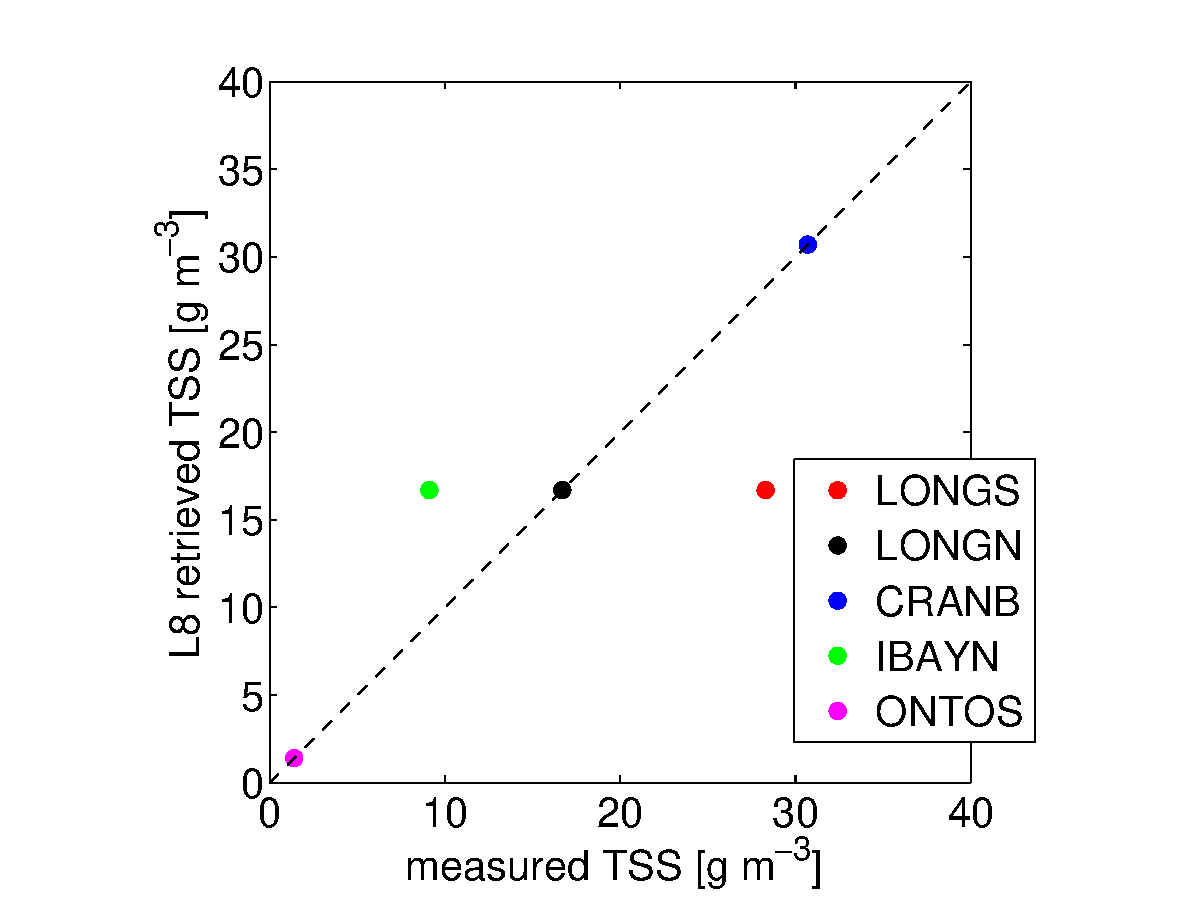
\includegraphics[height=5.5cm]{./Images/TSSretvsmea140929_150420}
  % \end{minipage}

%% CDOM
  \begin{minipage}[c]{1.0\linewidth}
  		\centering
      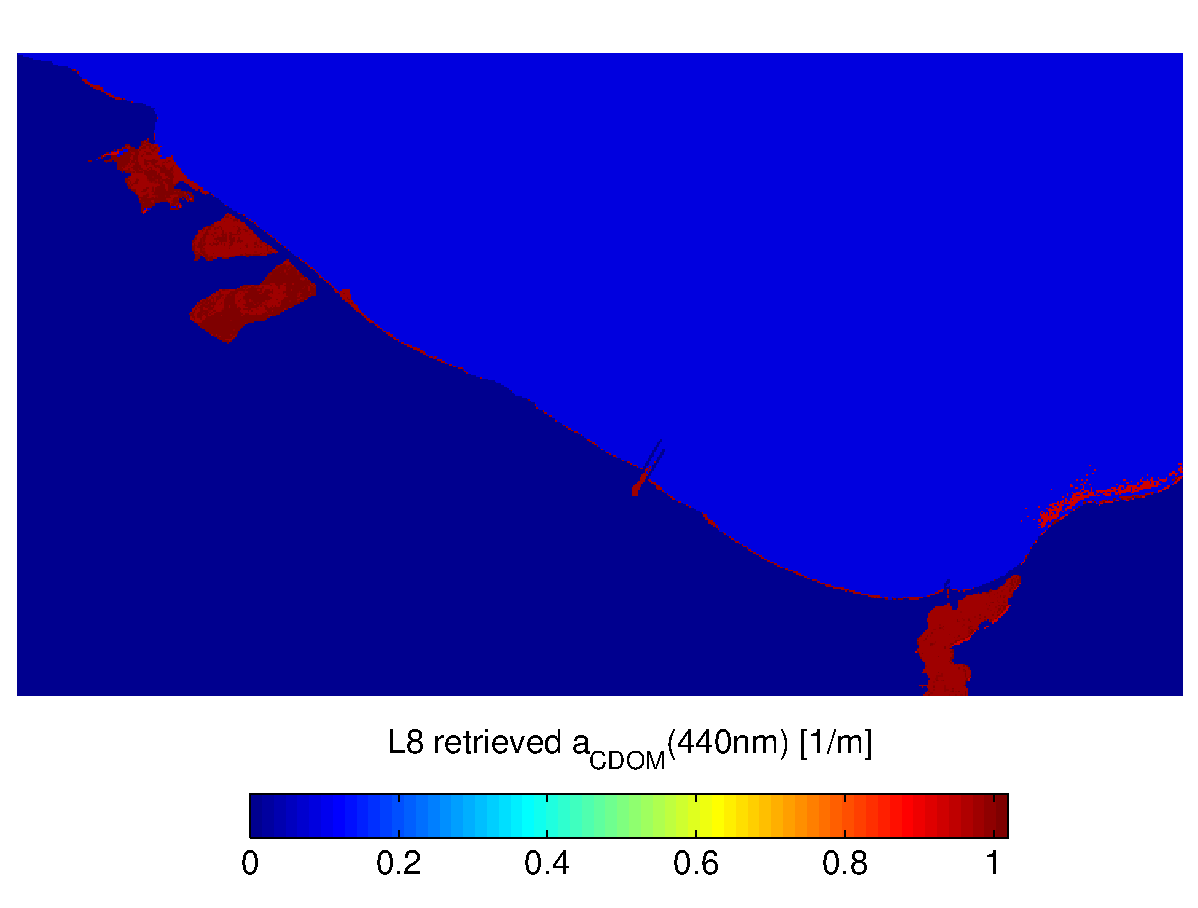
\includegraphics[trim=0 0 0 30,clip,height=7cm]{./Images/CDOMmap140929_150420}  
  \end{minipage}\\
  % \hfill
  % \begin{minipage}[d]{0.45\linewidth}
      % 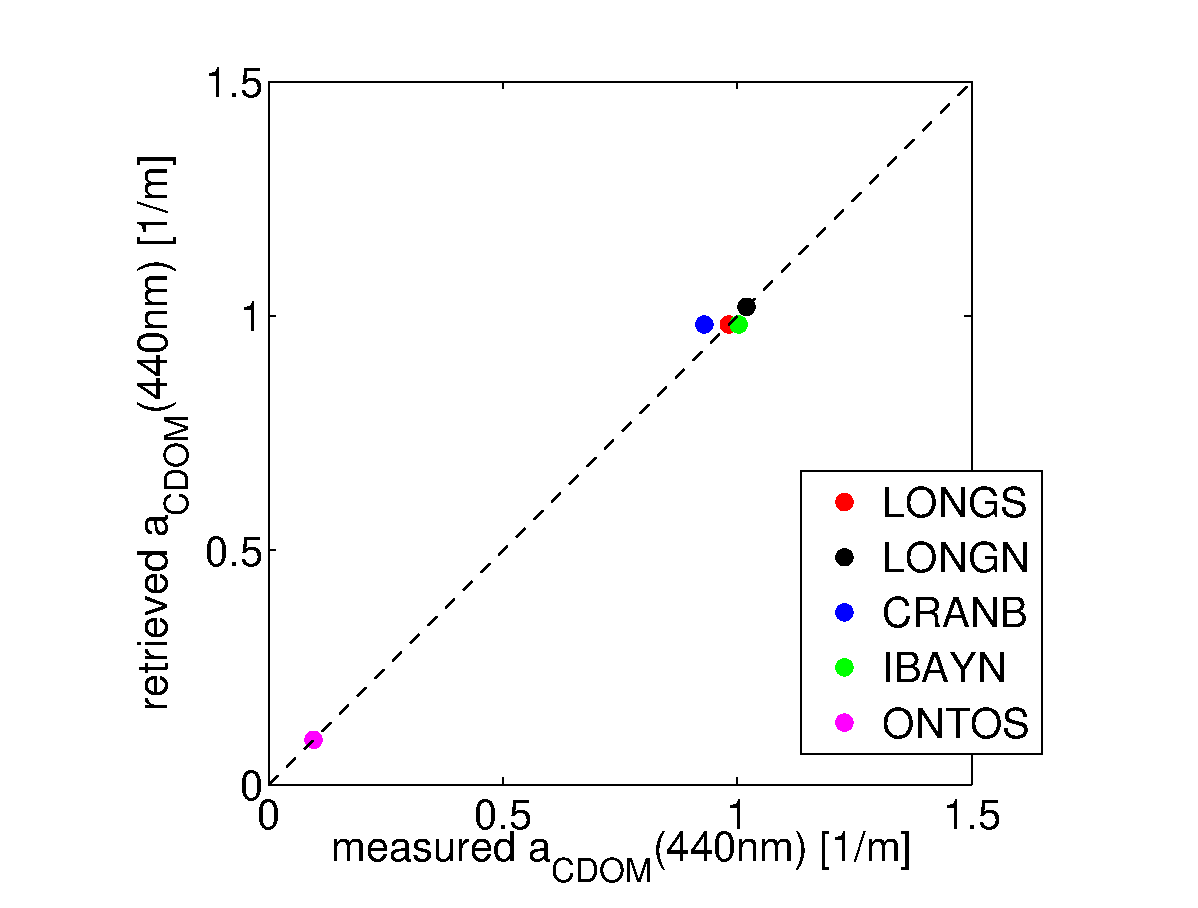
\includegraphics[height=5.5cm]{./Images/CDOMretvsmea140929_150420}
  % \end{minipage}

  \caption{CPA concentration maps for Landsat 8 image acquired on 09-29-2014 (scene LC80170302014272LGN00).\label{fig:CPAsMaps140929} } 
\end{figure}

% %%%%%%%%%%%%%%%%%%% SECTION %%%%%%%%%%%%%%%%%%%%%%%%%%%%%%%%
% \section{Discussion}

% Note that the image to be analyzed needs to only include a bright target and not necessary a big urban area in order to determine the bright pixel from the Landsat surface reflectance product.\\

A second image acquired on 09-29-2014 (scene LC80170302014272LGN00) (\autoref{fig:092914Sites}) was analyzed in a similar fashion except that the reflectance of the bright pixel target was also predicted by Ecolight using data for the most eutrophic pond (Cranberry Pond). This approach is attractive when a wide range of water quality conditions are present and concentration measurements are available of bright and dark water targets. This approach may improve results where glint is present as it compensates for not only atmospheric effects but any other approximately linear phenomena that would modify the reflected energy leaving the water volume. Note that glint effects were not specifically compensated for in the atmospheric correction process and future efforts using the urban region bright target approach will need to compensate for glint when it is present. The concentration maps for this second scene are illustrated in \autoref{fig:CPAsMaps140929} again showing reasonable patterns in the lake and ponds. \autoref{fig:CPAsRetVSMea} shows the comparison between predicted and observed values for all sample sites on both days, along with a regression line fitted to the data and its respective goodness of fit values. The $R^2$ value of the regression for all CPAs are high. Note that dark targets on both days and the bright target on the 2014 date are forced to match by the MoB-ELM process. The results are very encouraging showing good quantitative agreement across a very wide range of concentrations. 

The numerical results are summarized in \autoref{fig:RMSE} where the root mean squared error (RMSE) in predicted concentration is normalized by the range in concentrations to estimate overall performance, i.e.

\begin{equation}
\label{eq:error_percentage}
	RMSE~percentage~of~range =\frac{\sqrt{\frac{1}{N}\sum_{n=1}^N{\left[C_{ret}(n) - C_{mea}(n)\right]^2}}}{max\{C_{mea}(n)\} - min\{C_{mea}(n)\}}\times100 ~[\%]
\end{equation}

\noindent where $C_{ret}$ is the retrieved CPA concentration (i.e. $C_a$, $TSS$ or $a_{CDOM}(440nm)$), $C_{mea}$ is the measured CPA concentration, and $n=1,...,N$ is the $n$th site from a total of $N$ sites for both days. The RMSE percentage of range values are approximately $10\%$ for $C_a$ and $TSS$, and about $5\%$ for $a_{CDOM}(440nm)$. These errors are consistent with the expected errors reported by \cite*{Gerace:2013}. 

%%%%%%%%%%%%%%%%%%%%%%%%%%%%%%%%%%%%%%%%%%%%%%%%%%%%%%%%%%%%%%
\begin{figure}[htb]
  \begin{minipage}[c]{0.32\linewidth}
  % CHL
      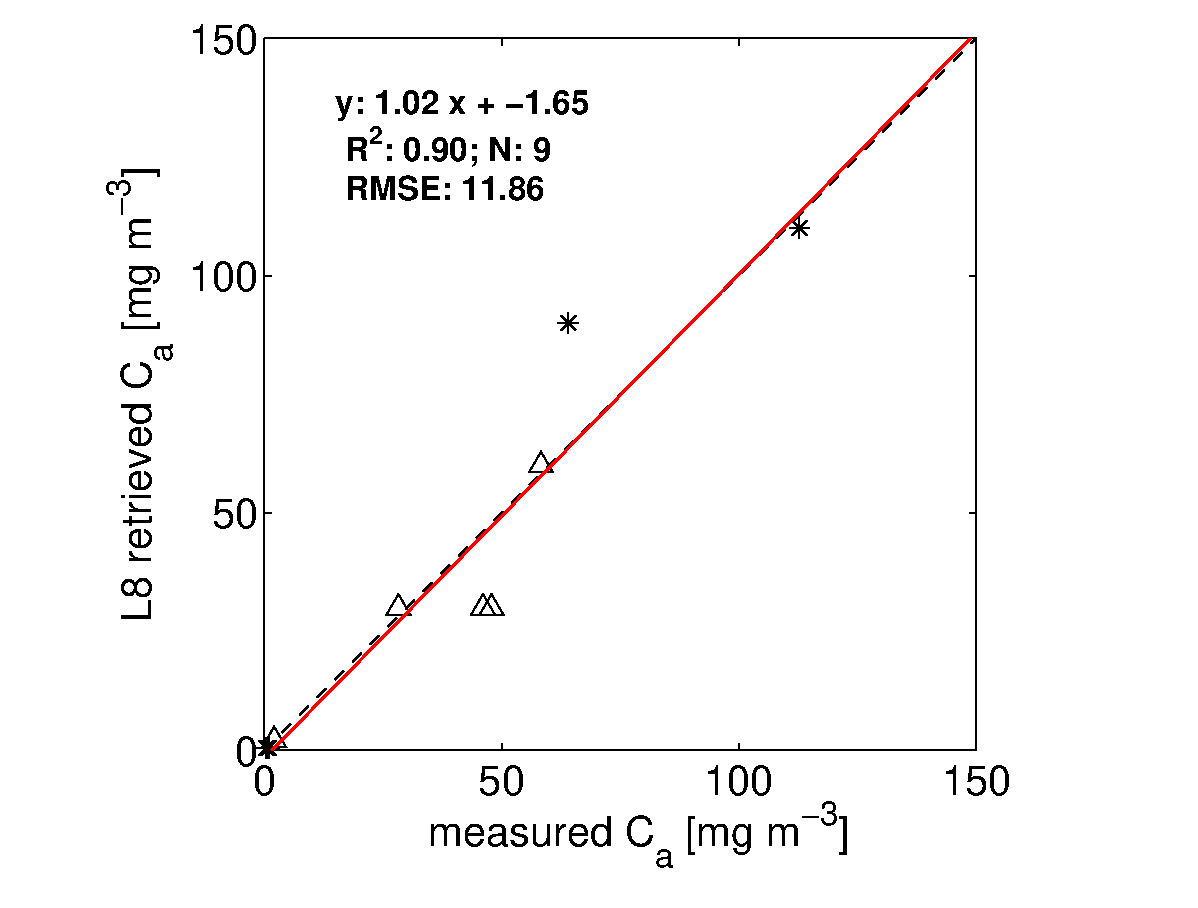
\includegraphics[trim=40 0 80 0,clip,height=5.1cm]{./Images/CHLretvsmea150423}  
  \end{minipage}
  % TSS
  \begin{minipage}[d]{0.32\linewidth}
      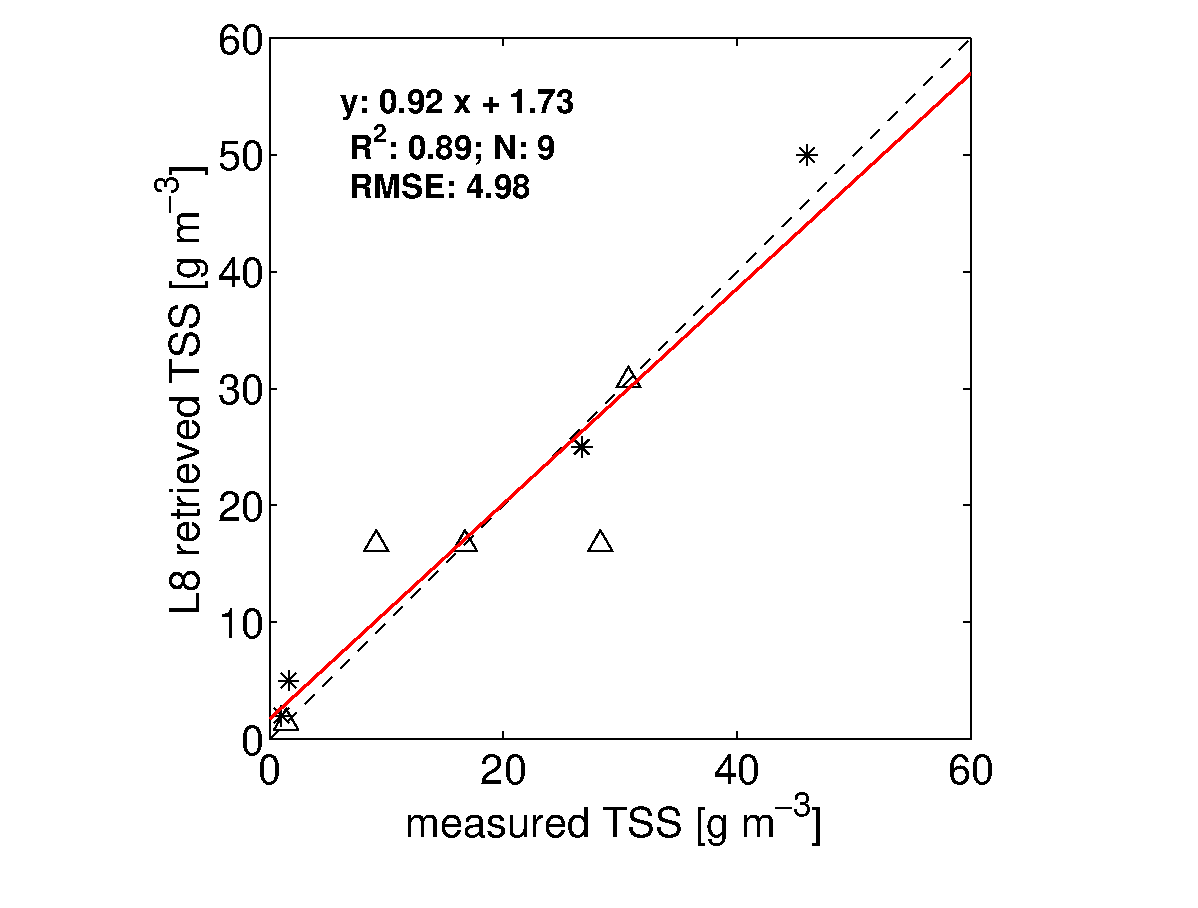
\includegraphics[trim=40 0 80 0,clip,height=5.1cm]{./Images/TSSretvsmea150423}
  \end{minipage}
  % CDOM
  \begin{minipage}[c]{0.32\linewidth}
      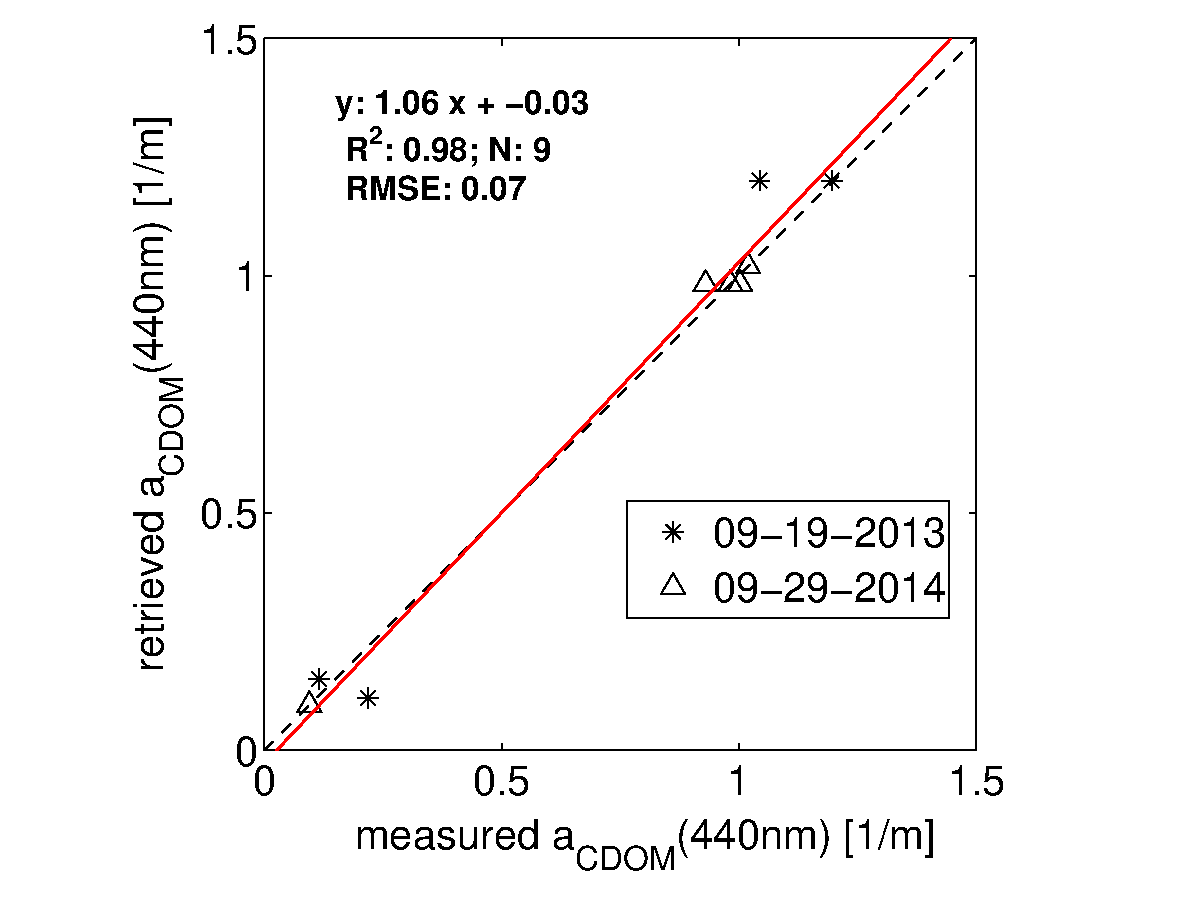
\includegraphics[trim=40 0 80 0,clip,height=5.1cm]{./Images/CDOMretvsmea150423}  
  \end{minipage}

  \caption{Landsat 8's retrieved vs measured CPA concentration for the 09-19-2014 and 09-29-2015 scenes with regression line (solid red line) and goodness of fit values. The dashed line represents the 1:1 line. \label{fig:CPAsRetVSMea} } 
\end{figure}

%%%%%%%%%%%%%%%%%%%%%%%%%%%%%%%%%%%%%%%%%%%%%%%%%%%%%%%%%%%%%%
\begin{figure}[htb]
	\centering
      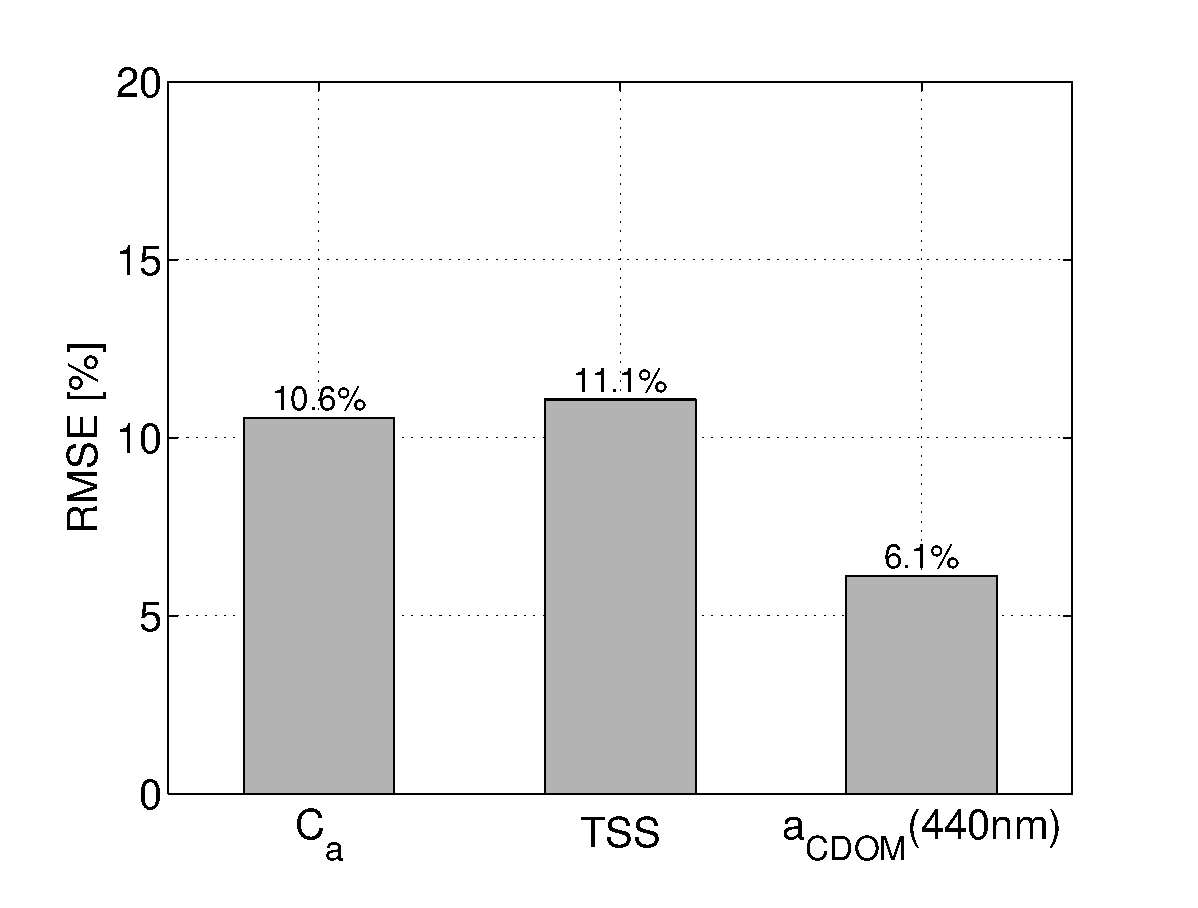
\includegraphics[height=5cm]{./Images/RMSE_ret150421}
      % \vspace{-.4cm}
      \caption{RMSE expressed as percentage of range for each CPA. \label{fig:RMSE}}
      % \vspace{-.4cm}
\end{figure}

%%%%%%%%%%%%%%%%%%% SECTION %%%%%%%%%%%%%%%%%%%%%%%%%%%%%%%%
\section{Conclusions}
The retrieval results shown in this study are promising for the use of Landsat 8 for monitoring of coastal and inland waters. The retrieval process was applied to two Landsat 8 scenes over the same study area and compared with field measurements. Maps of CPA concentrations show the expected trends of low concentration in the lake and higher concentration in the ponds. The retrieval was validated with ground-truth data taken at the same time as the satellite overpass, as opposed to comparison with historical field measurements. The comparison with field measurements exhibit error comparable with previous performance predictions for Landsat 8. An advantage of this retrieval algorithm is that it retrieves simultaneously all three CPAs.

The MoB-ELM atmospheric correction algorithm presented here tries to avoid the use of field reflectance ground-truth as commonly used in the traditional ELM method. In the MoB-ELM, the bright pixel is obtained from either the Landsat reflectance product over a bright target in the scene or from an Ecolight run simulating a water body with high concentration of CPAs in the scene. The dark pixel is obtained from an Ecolight run simulating a water body with low concentration of CPAs present in the scene. This algorithm does not require zero water signal in the NIR bands, so it could be applied to highly turbid waters. This algorithm assumes that the atmosphere is the same over the area of study.

 % and that the water signal in the SWIR bands is zero, which is commonly the case since water has a high absorption in the SWIR wavelengths, even in highly turbid waters
% Practical applications  
% Disadvantages and Advantages
% Limitations

One of the limitation of the developed retrieval algorithm is that the MoB-ELM needs some knowledge of the water body (e.g. IOPs and concentration of constituents at at least one point), which is often available but not always, and therefore, it will not work in every case because of the need for this knowledge. However, it is still a good answer for many cases where this knowledge is indeed available. Future work is aiming for an approach with good atmospheric correction without the need for ground-truth. For example, IOPs are often stable and could be estimated from previous studies (perhaps seasonally in some water bodies).

% Inclusion of a new red edge band in the future Landsat 9 will improve the results. 
Some pixels from the lake shoreline include signal from the bottom causing outliers in the retrieval results since the bottom reflectance was not accounted for in the process. The next version of this retrieval algorithm should address this issue. Glint and adjacency effects were also not addressed in this work, and they could affect the atmospheric correction.

For further validation, this method needs to be applied to more scenes over the same area of study or to a different area of study where sufficient ground-truth data are available to increase the number of samples to be compared. Additionally, the results from the MoB-ELM and the retrieval algorithm will be compared with standard products derived from ocean color satellites.

To date, there are no other sources of free access, open to the international science community, satellite imagery with similar spatial resolution or similar standard product (e.g. MODIS chl-a product) to compare with. Therefore, a direct comparison of results from our approach with typical algorithms over water bodies smaller than one kilometer is not possible. This is a challenge that needs to be addressed since there is a particular interest from local communities for monitoring water bodies that are not resolvable by current ocean color satellites. This is the case of the ponds included in this study, which are less than one kilometer in size. This fact makes Landsat 8 a pioneer in the retrieval of water quality parameters over medium to small water bodies. This also opens a need for more field measurement collection (i.e. IOPs, $R_{rs}$ and concentrations) on a regular basis where water quality needs to be assessed for the validation of products derived from moderate spatial resolution sensors such a Landsat 8 and the upcoming Sentinel 2. 
% Challenges

%%%%%%%%%%%%%%%%%%% SECTION %%%%%%%%%%%%%%%%%%%%%%%%%%%%%%%%
% \vspace{-.4cm}
\section*{Acknowledgments}
\vspace{-.2cm}
The authors would like to extend a special thanks to the United States Geological Survey (USGS) for its sponsorship (contract number G12PC00065) that has made this effort possible. Special thanks to the Monroe County Environmental Laboratory of the Monroe County Department of Environmental Services for the $C_a$ and $TSS$ measurements used to validate our in house concentration measurements. Nina Raque\~{n}o is thanked for her invaluable help in the logistic of the field data collections, and faculty, staff and students at the Rochester Institute of Technology for helping in the data collection, especially Paul Romanczyk. Also, thanks to Dr. Christy Tyler for facilitating the Aquatic Ecology Lab at RIT for the $C_a$ measurements.
%%%%%%%%%%%%%%%%%%% SECTION %%%%%%%%%%%%%%%%%%%%%%%%%%%%%%%%
% \vspace{-.4cm}
\section*{References}

%%%%%%%%%%%%%%%%%%%%%%%
%% Elsevier bibliography styles
%%%%%%%%%%%%%%%%%%%%%%%
%% To change the style, put a % in front of the second line of the current style and
%% remove the % from the second line of the style you would like to use.
%%%%%%%%%%%%%%%%%%%%%%%

%% Numbered
%\bibliographystyle{model1-num-names}

%% Numbered without titles
%\bibliographystyle{model1a-num-names}

%% Harvard
% \bibliographystyle{model2-names.bst}\biboptions{authoryear}

%% Vancouver numbered
%\usepackage{numcompress}\bibliographystyle{model3-num-names}

%% Vancouver name/year
%\usepackage{numcompress}\bibliographystyle{model4-names}\biboptions{authoryear}

%% APA style
\bibliographystyle{model5-names}\biboptions{authoryear}

%% AMA style
%\usepackage{numcompress}\bibliographystyle{model6-num-names}

%% `Elsevier LaTeX' style
% \bibliographystyle{elsarticle-num}
% \bibliographystyle{apalike}
\bibliography{javier_bib}


\end{document}